\chapter{The Two-Body Problem}
	
\section{Central Force Problem and Conservation Laws}

\subsection{Central force problem}
	A central force acts along the line joining two particles and depends only on their separation $r=|\vecx_1-\vecx_2|$. Such a force is a gradient of a scalar potential $V(r)$:
	\[
	\vecF(\vecx_1,\vecx_2) = \nabla V(r).
	\]
	Newton's equations for the pair are
	\begin{equation}
		\frac{d^2}{dt^2}\begin{bmatrix}m_1 & 0\\0&m_2\end{bmatrix}\begin{bmatrix}\vecx_1\\\vecx_2\end{bmatrix}
		=\begin{bmatrix}-\nabla V(r)\\ \nabla V(r)\end{bmatrix}. \label{eq:eom2}
	\end{equation}
	Six second-order ODEs $\Rightarrow$ 12 constants of integration in the general solution.
	
	\subsection{Separating centre-of-mass motion}
	\label{sec:com_separation}
	With $M=m_1+m_2$, $\mu = m_1m_2/M$, transform to relative and centre-of-mass coordinates,
	\[
	\begin{bmatrix}\vecr\\ \vec X\end{bmatrix}=\begin{bmatrix}1&-1\\ m_1/M& m_2/M\end{bmatrix}\begin{bmatrix}\vecx_1\\\vecx_2\end{bmatrix},
	\qquad
	\begin{bmatrix}\vecx_1\\\vecx_2\end{bmatrix}=\begin{bmatrix}m_2/M&1\\-m_1/M&1\end{bmatrix}\begin{bmatrix}\vecr\\\vec X\end{bmatrix}.
	\]
	Substituting into \eqref{eq:eom2} and left-multiplying by $\begin{bmatrix}m_2/M&-m_1/M\\1&1\end{bmatrix}$ diagonalizes the mass matrix and decouples the two sectors:
	\begin{align}
		\mu\,\ddot{\vecr} &= -\nabla V(r), \label{eq:relEOM}\\
		M\,\ddot{\vec X} &= 0. \label{eq:comEOM}
	\end{align}
	Equation \eqref{eq:comEOM} integrates trivially: $\vec X(t) = (\vec P/M)t+\vec X_0$, with $\vec P,\vec X_0$ six constants fixing the inertial frame in which the barycentre is at rest at the origin. Everything of dynamical interest is in the \emph{relative} coordinate $\vecr$, governed by \eqref{eq:relEOM} — a one-body central-force problem with reduced mass $\mu$.
	
	\subsection{Conserved quantities}
	
	\paragraph{Angular momentum.} Define $\vecL=\vecr\times\vecp=\mu\,\vecr\times\dot{\vecr}$. Then, because we are considering central force $\ddot{\vec r}\propto \hat{r}$ and hence,
	\[
	\dot{\vecL} = \mu\big[\dot{\vecr}\times\dot{\vecr}+\vecr\times\ddot{\vecr}\big]=0.
	\]
	$\vecL$ supplies three constants of motion: its magnitude $L$, and two angles fixing its direction — the \textbf{inclination} $\iota$ and \textbf{longitude of ascending node} $\Omega$ (Euler angles of the orbital plane relative to a reference plane). Conservation of $\vecL$ confines the motion to the plane $\perp\vecL$.
	
	\paragraph{Energy.} $E=K+V$ with $K=\tfrac12\mu\dot{\vecr}^2$ (the centre-of-mass kinetic term is a constant and drops out). Then
	\[
	\dot E = \mu\dot{\vecr}\cdot\ddot{\vecr}+\dot V
	=\mu\dot{\vecr}\cdot\ddot{\vecr}+\nabla V\cdot\dot{\vecr}
	=\big(\mu\ddot{\vecr}+\nabla V\big)\cdot\dot{\vecr}=0
	\]
	by \eqref{eq:relEOM}. So $E$ is conserved for \emph{any} central potential $V(r)$, not just gravity. Therefore, \textbf{total energy and angular momentum} constitutes four constant of integration. We will learn that there is one more, known as Runge Lenz vector which points towards periapsis and hence encodes the orientation of periapsis and the last constant of integration which is needed specifies the initial phase of the relative orbit ($t_p$)
	\[
	\underbrace{\mathbf R_0,\mathbf V_{\rm CM}}_{6}
	+
	\underbrace{a,e,i,\Omega,\omega,t_p}_{6}
	=12.
	\]
	
	\section{Coordinate Systems and Orbital Elements}
	\label{sec:coord_orbital_elements}

	Fix an equatorial (reference) frame with $\hat\Upsilon$ (vernal equinox / first point of Aries) along $X$ and celestial north $\hat N$ along $Z$; $\hat Y$ completes the right-handed triad. For a source at $(\mathrm{RA},\mathrm{DEC})=(\alpha,\delta)$ the line of sight is
	\[
	\hat R = \cos\delta\cos\alpha\,\hat\Upsilon+\cos\delta\sin\alpha\,\hat Y+\sin\delta\,\hat N,
	\]
	with in-sky-plane axes (pointing along increasing RA, DEC)
	\[
	\hat\alpha=\frac{\pdv{\hat R}{\alpha}}{\abs{\pdv{\hat R}{\alpha}}}=-\sin\alpha\,\hat\Upsilon+\cos\alpha\,\hat Y,\qquad
	\hat\delta=\frac{\pdv{\hat R}{\delta}}{\abs{\pdv{\hat R}{\delta}}}=-\sin\delta\cos\alpha\,\hat\Upsilon-\sin\delta\sin\alpha\,\hat Y+\cos\delta\,\hat N.
	\]
	
	The orbital plane has its own frame: origin at the barycentre, $X$-axis along the \textbf{line of nodes} (through the ascending node and the descending node), $Z$-axis along $\vecL$. Denote the unit vector towards the ascending node by $\hatn$. Then (doing anticlockwise passive rotation)
	
	\begin{equation}
		\begin{pmatrix} \hatn\\ \hat y\\ \hat L \end{pmatrix} =
		\begin{pmatrix} 1&0&0\\ 0&\cos\iota&\sin\iota\\ 0&-\sin\iota&\cos\iota \end{pmatrix} \begin{pmatrix} \cos\Omega&\sin\Omega&0\\ -\sin\Omega&\cos\Omega&0\\ 0&0&1 \end{pmatrix} \begin{pmatrix} \hat\alpha\\ \hat\delta\\ \hat R \end{pmatrix}.
		\label{eq:orbital_frame_rotation}
	\end{equation}
	Hence,
	\begin{align}
		\hatn  &= \cos\Omega\,\hat\alpha+\sin\Omega\,\hat\delta, \label{eq:node}\\
		\hat y &= -\sin\Omega\cos\iota\,\hat\alpha+\cos\Omega\cos\iota\,\hat\delta+\sin\iota\,\hat R, \label{eq:yhat}\\
		\hat L &= \sin\Omega\sin\iota\,\hat\alpha-\cos\Omega\sin\iota\,\hat\delta+\cos\iota\,\hat R, \label{eq:Lhat}
	\end{align}
	\begin{figure}[htbp]
		\centering
		\tdplotsetmaincoords{70}{120}
		\resizebox{\textwidth}{!}{
			
\includegraphics{fig_ch6_orbital_frame_3d.pdf}}
		\caption{Orientation of an orbit relative to sky plane. $\Omega$ (longitude of ascending node) is measured from the reference direction $\alpha$ to the ascending node along the sky plane; $\omega$ (argument of periapsis) is measured from the ascending node to perigee \emph{within} the orbital plane; $\iota$ (inclination) is the dihedral angle between the two planes, read off at the node; $\nu$ (true anomaly) is measured from perigee to the heavenly body's current position. This is exactly $(\Omega,\iota,\omega)$ of Eqs.~\eqref{eq:node}--\eqref{eq:yhat} describe.}
		\label{fig:elements}
	\end{figure}
	so that $\iota=\arccos(\hat L\cdot\hat R)$ is the angle between orbital and reference planes, and $(\hatn,\hat y,\hat L)$ is a right-handed orthonormal triad spanning the orbital plane plus its normal. In this plane use polar coordinates $(r,\phi)$ measured from $\hatn$:
	
	\begin{equation}
		\rhat=\cos\phi\,\hatn+\sin\phi\,\hat y,\qquad
		\phihat=-\sin\phi\,\hatn+\cos\phi\,\hat y. \label{eq:rhat_phihat}
	\end{equation}
	\paragraph{The projected orbit in the sky plane}: If the object in its orbital plane as the coordinate $(r\cos(\omega+\nu),r\sin(\omega+\nu))$, the corresponding coordinate in the sky plane could be found as (clockwise passive rotation):
	
	\begin{align}
		\begin{pmatrix}
			X \\
			Y \\
			Z
		\end{pmatrix}_{\text{Sky Plane}}= 
		\begin{pmatrix}
			\cos\Omega & -\sin\Omega & 0 \\
			\sin\Omega & \cos\Omega & 0 \\
			0 & 0 & 1
		\end{pmatrix}
		\begin{pmatrix}
			1 & 0 & 0 \\
			0 & \cos i & -\sin i \\
			0 & \sin i & \cos i
		\end{pmatrix}
		\begin{pmatrix}
			r\cos(\omega+\nu) \\
			r\sin(\omega+\nu) \\
			0
		\end{pmatrix}_{\text{Orbital Plane}}.
	\end{align}
	Then,
	\begin{align}
		X &= r\left(\cos(\omega+\nu)\cos\Omega-\sin (\omega+\nu)\sin\Omega\cos i\right),\\
		Y &= r\left(\cos(\omega+\nu)\sin\Omega+\sin (\omega+\nu)\cos\Omega\cos i\right).
	\end{align}
	\begin{figure}[htbp]
		\centering
		
\includegraphics{fig_ch6_conic_sections_geometry.pdf}
		\caption{In this North becomes the local $X$ axis and West becomes the $Y$ axis of the sky plane.}	
	\end{figure}
	
	One can set $\Omega=0$ by another set of basis in the sky plane and then the analysis simplifies immensely
	\begin{align}
		X &= r\cos(\omega+\nu),\\
		Y &= r\sin (\omega+\nu)\cos i.
	\end{align}
	We find that the semi minor axis shrinks by the factor of $\cos i$.
	\paragraph{The six orbital elements.} As the orbit solution unfolds below, six constants emerge in total: $\Omega,\iota$ (orientation of the plane, from $\vecL$), $a,e$ (size and shape, from $E,L$), $\omega$ (orientation of the ellipse \emph{within} the plane, the \textbf{argument of periapsis}), and $T_0$ (time of periapsis passage, fixing where on the ellipse the body is at a given time). Figure~\ref{fig:elements} shows all of these together.
	
	\section{Planar Motion and Kepler's Second Law}
	
	\paragraph{Areal velocity.} The area swept by $\vecr$ in time $dt$ is $dA=\int_{0}^{2\pi}\int_{0}^{r(\phi)} r drd\phi=\frac{1}{2}\int_{0}^{2\pi}r^2(\phi)d\phi$, so
	\begin{equation}
		\frac{dA}{dt}=\frac{r^2\dot\phi}{2} = \frac{L}{2\mu} = \text{const.} \label{eq:kepler2}
	\end{equation}
	This is \textbf{Kepler's second law}: equal areas in equal times. It follows purely from $\vecL$ being conserved, i.e.\ from the force being central — no dependence on the specific form of $V(r)$.
	
	\paragraph{Equations of motion in $(r,\phi)$.} With $Z\parallel\vecL$ and $X\parallel\hatn$, $\vecr=r\rhat$, and
	\[
	\dot{\vecr}=\dot r\,\rhat+r\dot{\hat{r}}=\dot r\,\rhat+r\dot\phi\,\phihat,\qquad
	\ddot{\vecr}=\big(\ddot r-r\dot\phi^2\big)\rhat+\big(2\dot r\dot\phi+r\ddot\phi\big)\phihat.
	\]
	where we used $\nabla_{\mu}\mathbf{e}_{\nu}=\Gamma^{\alpha}_{\mu\nu}\mathbf{e}_{\alpha}$ which gives $\dv{\hat{r}}{t}=\pdv{\hat{r}}{\phi}\dot{\phi}=\dot{\phi}\Gamma_{\phi r}^{\mu}\mathbf{e}_{\mu}=\dot{\phi}\frac{\mathbf{e}_{\phi}}{r}=\dot{\phi}\hat{\phi}$. 
	\begin{figure}
		\centering
		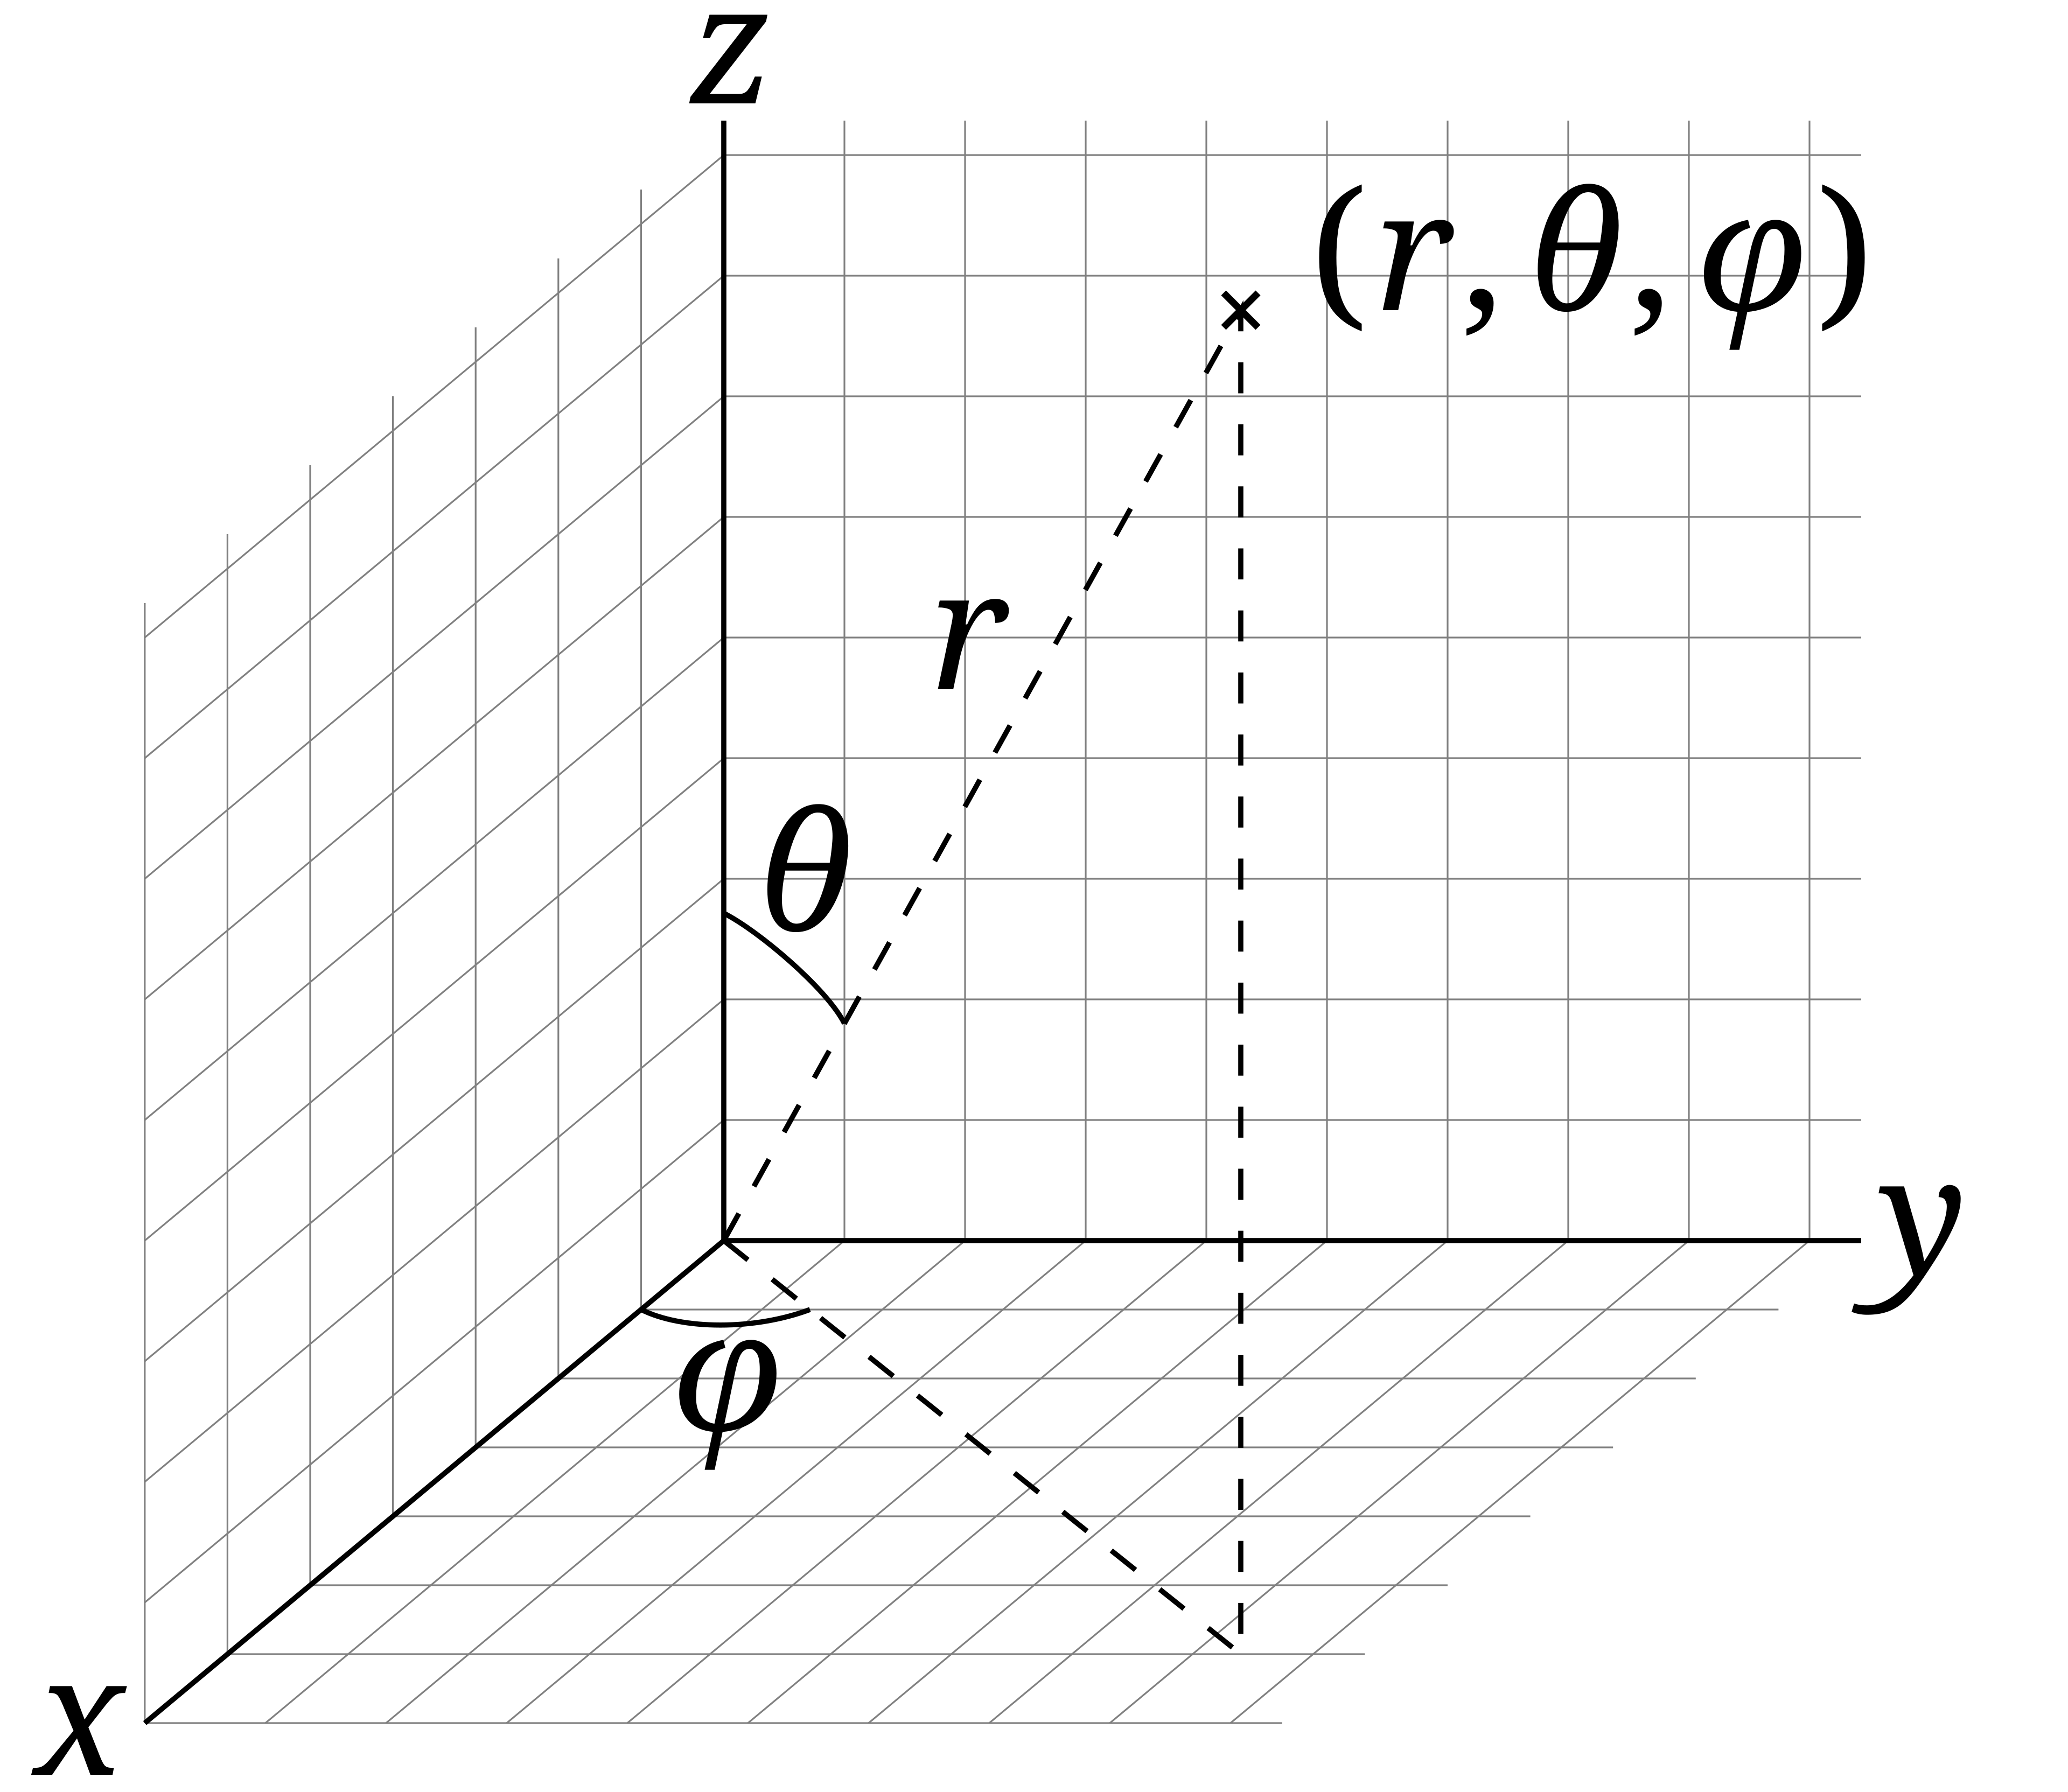
\includegraphics[width=0.5\linewidth]{3D_Spherical.png}
		\caption{Schematic description of spherical polar coordinates.}
		\label{fig:3D_spherical}
	\end{figure}
	Equation \eqref{eq:relEOM} splits into radial and tangential parts:
	\begin{align}
		\mu\big(\ddot r-r\dot\phi^2\big) &= -\nabla V(r), \label{eq:radial}\\
		\mu\big(2\dot r\dot\phi+r\ddot\phi\big) &= 0\implies \dv{(r^2\dot{\phi})}{t}=0. \label{eq:tangential}
	\end{align}
	This was supposed to be a coupled differential equation. But because of equation \eqref{eq:tangential} is just angular momentum conservation, i.e. Kepler's second law again, since $\vecL=\mu\vecr\times\dot{\vecr}=\mu r^2\dot\phi\,\hat L$. So
	\begin{equation}
		\dot\phi = \frac{L}{\mu r^2}, \label{eq:phidot}
	\end{equation}
	and \eqref{eq:radial} becomes, eliminating $\dot\phi$,
	\begin{equation}
		\mu\ddot r - \frac{L^2}{\mu r^3} = -\nabla V(r). \label{eq:radial_reduced}
	\end{equation}
	
	\section{The Orbit Equation}
	
	To get the orbit \emph{shape} $r(\phi)$ we change independent variable from $t$ to $\phi$ using \eqref{eq:phidot}: $\dfrac{dr}{dt}=\dot\phi\dfrac{dr}{d\phi}=\dfrac{L}{\mu r^2}\dfrac{dr}{d\phi}$, and
	\[
	\frac{d^2r}{dt^2}=\frac{L}{\mu r^2}\frac{d}{d\phi}\!\left[\frac{L}{\mu r^2}\frac{dr}{d\phi}\right]
	=\frac{L^2}{\mu^2 r^4}\left[\frac{d^2r}{d\phi^2}-\frac{2}{r}\left(\frac{dr}{d\phi}\right)^2\right].
	\]
	Substituting into \eqref{eq:radial_reduced} and dividing by $L^2/(\mu r^4)$:
	\[
	\frac{1}{r^4}\left[\frac{d^2r}{d\phi^2}-\frac{2}{r}\left(\frac{dr}{d\phi}\right)^2\right]-\frac{1}{r^3}=-\frac{\mu}{L^2}\nabla V(r).
	\]
	The standard trick is the \textbf{Binet substitution} $r=1/\rho$: then $dr/d\phi=-\rho^{-2}d\rho/d\phi$ and $d^2r/d\phi^2=-\rho^{-2}d^2\rho/d\phi^2+2\rho^{-3}(d\rho/d\phi)^2$. Substituting and simplifying (the $(d\rho/d\phi)^2$ terms cancel), one obtains the \textbf{orbit equation}:
	\begin{equation}
		\boxed{\frac{d^2\rho}{d\phi^2}+\rho = \frac{\mu}{L^2}\frac{1}{\rho^2}\nabla V\!\left(\frac1\rho\right).} \label{eq:orbiteq}
	\end{equation}
	This is a purely geometric ODE for the orbit's shape, valid for any central potential.
	
	\section{Keplerian Orbits}
	
	For Newtonian gravity, $V(r)=-GM\mu/r$, so $\nabla V(r) = GM\mu\rho^2\,\rhat$. Equation \eqref{eq:orbiteq} becomes
	\[
	\frac{d^2\rho}{d\phi^2}+\rho =\frac{GM\mu^2}{L^2}.
	\]
	
	Shifting $\tilde\rho=\rho-GM\mu^2/L^2$ turns this into the simple-harmonic-oscillator equation $\ddot{\tilde\rho}+\tilde\rho=0$ (derivatives in $\phi$), with solution $\tilde\rho=A\cos(\phi-\omega)$ for constants $A,\omega$. In terms of $r=1/\rho$:
	\[
	r(\phi)=\left(\frac{GM\mu^2}{L^2}+A\cos(\phi-\omega)\right)^{-1}
	=\frac{L^2/(GM\mu^2)}{1+\dfrac{L^2A}{GM\mu^2}\cos(\phi-\omega)}.
	\]
	Defining the \textbf{semi-latus rectum} $\lambda \equiv L^2/(GM\mu^2)$ as the value of $r$ when $\phi=\omega+90^{\circ}$ and \textbf{eccentricity} $e\equiv \lambda A$,
	\begin{equation}
		\boxed{r(\phi) = \frac{\lambda}{1+e\cos(\phi-\omega)}.} \label{eq:conic}
	\end{equation}
	This is the polar equation of a conic section with one focus at the origin, semi-latus rectum $\lambda$, eccentricity $e$, and major axis rotated by $\omega$ (the \textbf{argument of periapsis} — periapsis occurs at $\phi=\omega$). 
	\begin{figure}[htbp]
		\centering
		
		
		\usetikzlibrary{calc} %allows coordinate calculations
		
		% Newcommand
		
		%% Midline Label
		\newcommand{\midlinelabel}[3]{
			\node (midlabel) at ($ (#1)!.5!(#2) $) {#3};
			\draw[stealth-] (#1) --  (midlabel);
			\draw[-stealth] (midlabel) -- (#2);
		}
		%
		\newcommand{\midlinelabell}[3]{
			\node[fill = white, inner sep = 0.2pt, outer sep=3pt] (midlabel) at ($ (#1)!.5!(#2) $) {#3};
			\draw[stealth-] (#1) --  (midlabel);
			\draw[-stealth] (midlabel) -- (#2);
		}
		\newcommand{\midlinelabelll}[3]{
			\node[fill = white, inner sep = 0.2pt, outer sep=3pt,scale=0.6] (midlabel) at ($ (#1)!.5!(#2) $) {#3};
			\draw[stealth-] (#1) --  (midlabel);
			\draw[-stealth] (midlabel) -- (#2);
		}\usetikzlibrary{calc}
		
\includegraphics{fig_ch6_vis_viva_geometry.pdf}
	\end{figure}
	Two more shape parameters follow:
	\[
	a=\frac{\lambda}{1-e^2}\ \text{(semi-major axis)}, \qquad b = a\sqrt{1-e^2}\ \text{(semi-minor axis)}.
	\]
	One can check this directly from the equation of the ellipse,
	\begin{align}
		\frac{x^2}{a^2}+\frac{y^2}{b^2} &= 1,
	\end{align}
	by writing the polar coordinates about the focus as
	\begin{align}
		x &= ae+r(\phi)\cos\phi,\\
		y &= r(\phi)\sin\phi.
	\end{align}
	Substitution gives
	\begin{align}
		\frac{(ae+r\cos\phi)^2}{a^2}+\frac{r^2\sin^2\phi}{a^2(1-e^2)}&=1.
	\end{align}
	Solving for \(r\) then yields
	\begin{align}
		r(\phi)&=\frac{a(1-e^2)}{1+e\cos\phi}.
	\end{align}
	
	\begin{center}
		\begin{tabular}{@{}ll@{}}
			\toprule
			Eccentricity & Conic section\\
			\midrule
			$e=0$ & circle\\
			$0<e<1$ & ellipse ($E<0$, bound)\\
			$e=1$ & parabola ($E=0$)\\
			$e>1$ & hyperbola ($E>0$, unbound)\\
			\bottomrule
		\end{tabular}
	\end{center}
	Bound, closed elliptical orbits ($E<0$) constitute \textbf{Kepler's first law}. In the original (unreduced) frame,
	\[
	\vecx_1=\frac{m_2}{M}\vecr,\qquad \vecx_2=-\frac{m_1}{M}\vecr.
	\]
	
	\section{Energy and Angular Momentum in Terms of \texorpdfstring{$a,e$}{a,e}}
	
	\subsection{Energy}
	\[
	E=\frac12\mu\dot{\vecr}^2-\frac{GM\mu}{r} = \frac12\mu\big(\dot r^2+r^2\dot\phi^2\big)-\frac{GM\mu}{r}
	=\frac12\mu\dot r^2+\frac{L^2}{2\mu r^2}-\frac{GM\mu}{r}.
	\]
	Since $E$ is conserved, evaluate at periapsis ($\phi=\omega$), where $r=a-ae=\lambda/(1+e)$ and $\dot r=0$ (turning point of $r$):
	\[
	E = 0+\frac{L^2(1+e)^2}{2\mu\lambda^2}-\frac{GM\mu(1+e)}{\lambda}
	=\frac{GM\mu^2\lambda(1+e)^2}{2\mu\lambda^2}-\frac{GM\mu(1+e)}{\lambda}
	=-\frac{GM\mu}{2\lambda}(1-e^2),
	\]
	using $L^2=GM\mu^2\lambda$ (below). With $a=\lambda/(1-e^2)$,
	\begin{equation}
		\boxed{E=-\frac{GM\mu}{2a}.} \label{eq:visviva_E}
	\end{equation}
	Since $\lambda>0$ always, the sign of $E$ tracks $e$: bound orbits ($E<0$) have $e<1,\ a>0$; unbound orbits ($E\geq0$) have $e\geq1$; hyperbolic orbits formally have $a<0$.
	
	\subsection{Angular momentum}
	Both at apoapsis $(r=a+ae=\frac{\lambda}{1-e})$ and periapsis$(r=a-ae=\frac{\lambda}{1+e})$, we have $\dot{r}=0$,
	\begin{align}
		\frac{L^2(1+e)^2}{2\mu\lambda^2}-\frac{GM\mu(1+e)}{\lambda}
		=\frac{L^2(1-e)^2}{2\mu\lambda^2}-\frac{GM\mu(1-e)}{\lambda}
	\end{align}
	Solving for $L$:
	\begin{equation}
		L=\sqrt{GM\mu^2\lambda}, \qquad\text{i.e.}\qquad L^2=GM\mu^2 a(1-e^2), \label{eq:L_of_ae}
	\end{equation}
	and, using \eqref{eq:Lhat},
	\[
	\vecL = \sqrt{GM\mu^2\lambda}\,\big(-\sin\Omega\sin\iota\,\hat\alpha+\cos\Omega\sin\iota\,\hat\delta+\cos\iota\,\hat R\big).
	\]
	
	\subsection{Instantaneous kinetic energy}
	\label{sec:vis_viva}
	From $E=K+V$: $K=\tfrac12\mu\dot{\vecr}^2 = E-V= GM\mu\left(\dfrac1r-\dfrac1{2a}\right)$ — the \emph{vis-viva} equation. Splitting between the two bodies via $\vecx_i$: $K_1=\tfrac12 m_1v_1^2=\tfrac{m_2}{M}K$, $K_2=\tfrac{m_1}{M}K$.
	
	\paragraph{Inverting for $a,e$.} Equations \eqref{eq:visviva_E}--\eqref{eq:L_of_ae} give the orbital elements directly from the (conserved) energy and angular momentum:
	\begin{equation}
		a=-\frac{GM\mu}{2E},\qquad e=\sqrt{1+\frac{2EL^2}{(GM)^2\mu^3}}. \label{eq:a_e_from_EL}
	\end{equation}
	
	\section{True and Eccentric Anomaly; Kepler's Equation}
	
	We now want $r(t)$ (and hence $\phi(t)$), not just $r(\phi)$. From the vis-viva relation,
	\[
	\dot r = \sqrt{\frac{2}{\mu}\left(E-\frac{L^2}{2\mu r^2}+\frac{GM\mu}{r}\right)}
	=\sqrt{GM}\,\frac1r\left(2r-\frac{r^2}{a}-\lambda\right)^{1/2},
	\]
	using \eqref{eq:visviva_E}--\eqref{eq:L_of_ae} to trade $E,L$ for $a,\lambda$. Then
	\begin{align}
		\int_{t_0}^{t}dt&=\frac{1}{\sqrt{GM}}\int_{r_0}^{r}\frac{r'\,dr'}{\left(2r'-r'^2/a-\lambda\right)^{1/2}}\\
		t-t_0&=\sqrt{\frac{a}{GM}}\int_{r_0}^{r}\frac{r'dr'}{\sqrt{a^2e^2-(r'-a)^2}}\tag{using $\lambda=a(1-e^2)$}
	\end{align}
	\subsection{Elliptical orbits: eccentric anomaly}
	For $a>0$, substitute
	\begin{equation}
		r=a\big(1-e\cos u\big), \label{eq:r_of_u}
	\end{equation}
	where $u$ is the \textbf{eccentric anomaly} (this choice guarantees $r>0$ throughout, since $-1\le\cos u\le1$). Then $dr=ae\sin u\,du$, and the bracket under the square root simplifies to $a e^2\sin^2u$, so the square root is simply $\sqrt a\, e\,|\sin u|$. The integral collapses to
	\[
	t-t_0=\frac{a^{3/2}}{\sqrt{GM}}\int_0^u (1-e\cos u')\,du' = \frac{a^{3/2}}{\sqrt{GM}}\big[u-e\sin u\big],
	\]
	where $t_0$ (\textbf{epoch}) is the time at which $u=0$ — the sixth and final constant of integration, $T_0$.
	
	\paragraph{Relating true anomaly $v$ and eccentric anomaly $u$:}
	Define the \textbf{true anomaly} $v\equiv\phi-\omega$ (so $r=\lambda/(1+e\cos v)$ from \eqref{eq:conic}). Equating this with \eqref{eq:r_of_u}:
	\[
	\frac{1-e\cos u}{1-e^2}=\frac{1}{1+e\cos v}
	\quad\Longrightarrow\quad
	\cos v = \frac{\cos u - e}{1-e\cos u}. \tag{65a}
	\]
	Consistently,
	\begin{equation}
		\sin v = \frac{\sqrt{1-e^2}\sin u}{1-e\cos u},\qquad
		\tan v = \frac{\sqrt{1-e^2}\sin u}{\cos u - e},\qquad
		\tan\frac v2 = \sqrt{\frac{1+e}{1-e}}\,\tan\frac u2. \label{eq:v_of_u}
	\end{equation}
	At $u=0$ and $u=\pi$, $v=u$ — periapsis and apoapsis coincide for the two anomalies, as they must by symmetry.
	
	\subsection{Hyperbolic trajectories}
	For $a<0$ (and $e>1$), the analogous substitution is $r=a(1-e\cosh u)$ (using $\cosh u\ge1$ keeps $r>0$ since $a<0$). Carrying through the same integral gives the \textbf{hyperbolic} anomaly relation
	\[
	t-t_0 = \frac{(-a)^{3/2}}{\sqrt{GM}}\big[e\sinh u - u\big],
	\]
	with true-anomaly relations
	\begin{equation}
		\cos v = \frac{e-\cosh u}{e\cosh u - 1},\qquad
		\sin v = \frac{\sqrt{e^2-1}\sinh u}{e\cosh u-1},\qquad
		\tan\frac v2=\sqrt{\frac{e+1}{e-1}}\tanh\frac u2. \label{eq:v_of_u_hyp}
	\end{equation}
	
	\section{Kepler's Third Law}
	
	For one complete orbit, $u$ advances by $2\pi$ while $t$ advances by the orbital period $2\pi/n$ ($n\equiv$ mean motion):
	\begin{equation}
		\frac{2\pi}{n} = \frac{a^{3/2}}{\sqrt{GM}}\big[2\pi - e\sin(2\pi)\big] = \frac{a^{3/2}}{\sqrt{GM}}\cdot2\pi
		\quad\Longrightarrow\quad
		\boxed{n=\sqrt{\frac{GM}{a^3}},\qquad n^2a^3=GM.} \label{eq:kepler3}
	\end{equation}
	
	\section{Kepler's Equation}
	\label{sec:kepler_equation}

	Substituting $n=\sqrt{GM/a^3}$ into $t-t_0=(a^{3/2}/\sqrt{GM})(u-e\sin u)$ and defining the \textbf{mean anomaly} $\ell\equiv n(t-t_0)$:
	\begin{equation}
		\boxed{\ell = u - e\sin u} \qquad\text{(elliptical Kepler's equation).} \label{eq:kepler_eq}
	\end{equation}
	This transcendental equation must be solved numerically (or by series, \S\ref{sec:bessel}) for $u(\ell)$, i.e.\ $u(t)$. The hyperbolic analogue (with $n\equiv GM/(-a)^{3/2}$) is
	\begin{equation}
		\ell = e\sinh u - u. \label{eq:kepler_eq_hyp}
	\end{equation}
	
	\section{Keplerian Parametrization}
	\label{sec:parametrization}
	
	\subsection{Elliptical orbits}
	Collecting results:
	\begin{align}
		r&=a(1-e\cos u), & \phi&=v+\omega,\\
		\tan\frac v2 &= \sqrt{\frac{1-e}{1+e}}\tan\frac u2, & \ell&=u-e\sin u.
	\end{align}
	
	Differentiating Kepler's equation \eqref{eq:kepler_eq} in $t$: $n=\dot u(1-e\cos u)$, so
	\begin{equation}
		\dot u = \frac{n}{1-e\cos u}. \label{eq:udot}
	\end{equation}
	Differentiating $r=a(1-e\cos u)$:
	\begin{equation}
		\dot r = ae\sin u\,\dot u = \frac{an\,e\sin u}{1-e\cos u}. \label{eq:rdot_u}
	\end{equation}
	Differentiating the $v$-$u$ relation and using \eqref{eq:v_of_u}, one finds $dv/du = \sqrt{1-e^2}/(1-e\cos u)$, so
	\begin{equation}
		\dot\phi = \dot v = \frac{dv}{du}\dot u = \frac{n\sqrt{1-e^2}}{(1-e\cos u)^2}. \label{eq:phidot_u}
	\end{equation}
	
	\subsection{Hyperbolic trajectories}
	Analogously, with $r=-a(e\cosh u - 1)$, $\phi=v+\omega$, $\tan(v/2)=\sqrt{(e+1)/(e-1)}\tanh(u/2)$, $\ell=e\sinh u - u$:
	\begin{equation}
		\dot u = \frac{n}{e\cosh u - 1},\quad
		\dot r = -an\,\frac{e\sinh u}{e\cosh u - 1},\quad
		\dot\phi=\dot v = \frac{n\sqrt{e^2-1}}{(e\cosh u-1)^2}. \label{eq:hyp_derivs}
	\end{equation}
	
	\section{Hyperbolic-Trajectory Parameters}
	
	For unbound ($e>1$) encounters, four derived quantities are standard:
	
	\textbf{Hyperbolic excess velocity} $v_\infty$: from $\tfrac12\mu\dot{\vecr}_\infty^2 = -GM\mu/(2a)$ (recall $a<0$),
	\begin{equation}
		|\dot{\vecr}_\infty| = \sqrt{-\frac{GM}{a}}. \label{eq:vinf}
	\end{equation}
	
	\textbf{Scattering angle} $\theta_\infty$: half the angle between the two asymptotes,
	\begin{equation}
		\cos\theta_\infty = -\lim_{u\to\infty}\frac{e-\cosh u}{e\cosh u -1} = \frac1e. \label{eq:scattering}
	\end{equation}
	
	\textbf{Periapsis distance}:
	\begin{equation}
		r_p = \min_v \frac{a(1-e^2)}{1+e\cos v} = -a(e-1). \label{eq:rp}
	\end{equation}
	
	\textbf{Semi-minor axis / impact parameter}: the semi-minor axis $b=-a\sqrt{e^2-1}$ satisfies $-ab=\lambda$. The impact parameter $b'$ (miss distance of the unperturbed asymptote) is
	\[
	b' = (-a+r_p)\sin\theta_\infty = -ae\sin\theta_\infty = -a\sqrt{e^2-1} = b,
	\]
	i.e.\ impact parameter and semi-minor axis coincide.
	
	\textbf{Flight-path angle} (angle between $\dot{\vecr}$ and the direction $\perp\rhat$ in-plane):
	\begin{equation}
		\sin\varphi = \frac{\dot{\vecr}\cdot\rhat}{|\dot{\vecr}|}=\frac{\dot r}{\sqrt{\dot r^2+r^2\dot\phi^2}}. \label{eq:flightpath}
	\end{equation}
	
	\section{Fourier Solution of Kepler's Equation}
	\label{sec:bessel}
	
	Kepler's equation $u-\ell=e\sin u$ can be solved as a Fourier series in $\ell$:
	\[
	e\sin u = \sum_{s=1}^{\infty}A_s\sin(s\ell).
	\]
	Using $A_s = \tfrac2\pi\int_0^\pi (u-\ell)\sin(s\ell)\,d\ell$, integrating by parts (the boundary term vanishes since $u=\ell$ at $\ell=0,\pi$), and substituting $d\ell = (1-e\cos u)\,du$ (from Kepler's equation) turns the $\ell$-integral into a $u$-integral:
	\[
	A_s = \frac{2}{s\pi}\int_0^\pi \cos(su-se\sin u)\,du = \frac{2}{s}J_s(se),
	\]
	recognizing the integral representation of the Bessel function of the first kind, $J_s(x)=\tfrac1\pi\int_0^\pi\cos(s\tau-x\sin\tau)\,d\tau$. So
	\begin{equation}
		u(\ell) = \ell + \sum_{s=1}^{\infty}\frac{2}{s}J_s(se)\sin(s\ell). \label{eq:kepler_series}
	\end{equation}
	This is the classical Bessel-function series solution to Kepler's equation.
	
	\section{The Laplace--Runge--Lenz Vector}
	
	Define $\vecA \equiv \vecp\times\vecL - GM\mu^2\rhat$ (with $\vecp=\mu\dot{\vecr}$). For the pure Kepler problem,
	\[
	\dot{\vecA} = \dot{\vecp}\times\vecL - GM\mu^2\dot{\rhat}
	= -\frac{GM\mu}{r^2}\big(\rhat\times\vecL\big) - GM\mu^2\dot\phi\,\phihat.
	\]
	Using $\vecL=L\hat L$, planar motion identities $\rhat\times\hat L=-\phihat$, and $\dot\phi=L/(\mu r^2)$ from \eqref{eq:phidot}:
	\[
	\dot{\vecA} = -GM\mu\left(\frac{L}{r^2}\phihat - \mu\dot\phi\,\phihat\right)=0,
	\]
	so $\vecA$ is conserved for the unperturbed problem — it is a \emph{fourth}, non-obvious constant of the Kepler problem (beyond $E,\vecL$), reflecting the extra "hidden" $SO(4)$ symmetry of the $1/r$ potential.
	
	\paragraph{Direction and magnitude of $\vecA$.} From the definition it is clear that $\vecA$ is planar. Therefore, we can decompose it as $\vecA=A_r\hat{r}+A_{\phi}\hat{\phi}$.
	
	\begin{figure}[htbp]
		\centering
		\tdplotsetmaincoords{70}{115}
		
		
\includegraphics{fig_ch6_orbital_elements_3d.pdf}
		\caption{The Runge Lenz vector points radially outward at perigee. Since it is conserved, the direction and magnitude stays fixed during the entire evolution.}
	\end{figure}
	At periapsis the velocity is purely tangential ($\vecp\perp\rhat$), so $\rhat\times\vecA\big|_{\rm peri}=\rhat\times(\vecp\times\vecL)\big|_{\rm peri}=\big[\vecp(\rhat\cdot\vecL)-\vecL(\rhat\cdot\vecp)\big]_{\rm peri}=0$ (both dot products vanish there). Also $\rhat\cdot\vecA|_{\rm peri}=A$ (from the relation above with $v=0$ at periapsis). Together these mean $\hat A = \rhat|_{\rm peri}$: $\vecA$ points from the focus \emph{towards periapsis}.
	
	Since $\vecA$ points radially outwards at the Periapsis. We find the magnitude by doting $\vecA$ into $\vecr$:
	\begin{align}
		\vecA\cdot\vecr &= (\vecp\times\vecL)\cdot\vecr - GM\mu^2 r \\
		&=p_i L_j \epsilon_{ijk}r_k-GM\mu^2 r=p_i L_j \epsilon_{kij}r_k-GM\mu^2 r\\
		&= \underbrace{(\vecr\times\vecp)}_{\vecL}\cdot\vecL - GM\mu^2 r = L^2 - GM\mu^2 r,\end{align}
	i.e., writing $\vecA\cdot\vecr = Ar\cos v$ (with $v$ the angle between $\vecA$ and $\vecr$), using
	\[
	r = \frac{L^2/(GM\mu^2)}{1+e\cos v}\implies GM\mu^2 r = \frac{L^2}{1+e\cos v}.
	\]
	We find:
	\begin{align}
		Ar\cos v&=L^2 - GM\mu^2 r,\\
		A \frac{L^2/GM\mu^2}{1+e\cos v}\cos v&=L^2\left(1-\frac{1}{1+e\cos v}\right)=\frac{L^2e\cos v}{1+e\cos v}
	\end{align}
	
	Hence
	\begin{equation}
		\boxed{A = GM\mu^2 e.} \label{eq:A_magnitude}
	\end{equation}
	Using \eqref{eq:rhat_phihat}:
	\begin{equation}
		\hat A = \cos\omega\,\hatn+\sin\omega\,\hat y. \label{eq:Ahat}
	\end{equation}
	Equivalently, the \textbf{eccentricity vector} $\vec e \equiv \vecA/(GM\mu^2) = e\hat A=e(\cos\omega,\sin\omega,0)$ is a conserved vector encoding $(e,\omega)$ together. Since $e,\Omega,\iota$ are already determined by $(E,\vecL)$, the only \emph{new} information in $\vecA$ is $\omega$, i.e. the in-plane orientation of the ellipse or the direction of periapsis from the line of ascending node.
	
	\section{Perturbed Orbits}
	\label{sec:perturbed_orbits}
	
	We now allow an additional force $\vec F$ in the relative equation of
	motion:
	\begin{equation}
		\boxed{
			\mu\ddot{\vecr}
			=
			-\frac{GM\mu}{r^2}\rhat+\vec F .
		}
		\label{eq:perturbed_eom}
	\end{equation}
	The central Newtonian term defines the Kepler problem; $\vec F$ is the
	perturbing force and need not be central.
	
	The momentum is
	\begin{equation}
		\vecp=\mu\dot{\vecr},
	\end{equation}
	and, in the orbital plane,
	\begin{equation}
		\vecp
		=
		\mu\dot r\,\rhat+\frac{L}{r}\,\phihat,
		\qquad
		L=\mu r^2\dot\theta .
		\label{eq:polar_momentum}
	\end{equation}
	
	The purpose of orbital perturbation theory is to represent the actual
	trajectory by Keplerian orbital elements which vary with time, and to
	derive their rates directly from \eqref{eq:perturbed_eom}.
	
	\subsection{Osculating Kepler orbit}
	\label{sec:osculating_orbit}
	
	For $\vec F=0$, the Kepler solution can be written in terms of six
	constants
	\begin{equation}
		Q=(Q_1,\ldots,Q_6)
		=
		(a,e,\iota,\Omega,\omega,T_0),
	\end{equation}
	so that
	\begin{equation}
		\vecr=\vecr(Q,t),
		\qquad
		\vecp=\vecp(Q,t).
		\label{eq:kepler_phase_solution}
	\end{equation}
	For fixed $Q$, these functions satisfy the unperturbed equations of
	motion.
	
	For the perturbed problem, let
	\begin{equation}
		Q_i=Q_i(t).
	\end{equation}
	The actual trajectory is represented in terms of a set of
	time-dependent osculating orbital elements \(Q(t)\) as
	\begin{equation}
		\vecr(t)
		=
		\vecr_{\rm osc}\bigl(Q(t),t\bigr),
		\qquad
		\vecp(t)
		=
		\vecp_{\rm osc}\bigl(Q(t),t\bigr).
		\label{eq:perturbed_parameterization}
	\end{equation}
	Here, for fixed values of \(Q\), the functions
	\(\vecr_{\rm osc}(Q,t)\) and \(\vecp_{\rm osc}(Q,t)\) describe the
	corresponding Keplerian orbit.  The time dependence of \(Q(t)\) accounts
	for the slow evolution of this osculating Keplerian orbit under the
	perturbing force.
	
	At each instant, the osculating Kepler orbit is chosen to have the same
	position and momentum as the actual trajectory.  Thus,
	\begin{equation}
		\vecr_{\rm osc}\bigl(Q(t),t\bigr)=\vecr(t),
		\qquad
		\vecp_{\rm osc}\bigl(Q(t),t\bigr)=\vecp(t).
		\label{eq:osculating_state}
	\end{equation}
	Importantly, this representation does not imply that the actual
	trajectory is itself Keplerian.  Rather, it is represented at each
	instant by the Keplerian orbit that osculates it at that instant.
	
	The corresponding accelerations are different:
	\begin{align}
		\dot{\vecp}_{\rm actual}
		&=
		-\frac{GM\mu}{r^2}\rhat+\vec F,
		\\
		\dot{\vecp}_{\rm osc}
		&=
		-\frac{GM\mu}{r^2}\rhat.
	\end{align}
	Hence
	\begin{equation}
		\boxed{
			\dot{\vecp}_{\rm actual}
			-
			\dot{\vecp}_{\rm osc}
			=
			\vec F .
		}
		\label{eq:perturbation_acceleration_difference}
	\end{equation}
	
	The two trajectories therefore agree in position and momentum at the
	instant at which the osculating orbit is constructed, but they have
	different subsequent evolution.
	
	\subsection{Variation of parameters}
	
	Differentiating \eqref{eq:perturbed_parameterization},
	\begin{equation}
		\dot{\vecr}
		=
		\left.\pdv{\vecr}{t}\right|_Q
		+
		\sum_{i=1}^{6}
		\pdv{\vecr}{Q_i}\dot Q_i .
		\label{eq:r_chain_rule}
	\end{equation}
	For fixed $Q$, the first term is the velocity of the Kepler solution.
	The osculating condition requires this Kepler velocity to coincide with
	the actual velocity:
	\begin{equation}
		\dot{\vecr}
		=
		\left.\pdv{\vecr}{t}\right|_Q.
	\end{equation}
	Therefore
	\begin{equation}
		\boxed{
			\sum_{i=1}^{6}
			\pdv{\vecr}{Q_i}\dot Q_i=0 .
		}
		\label{eq:osculating_r_constraint}
	\end{equation}
	
	This is a vector equation and therefore supplies three scalar
	conditions.
	
	Now differentiate $\vecp(Q(t),t)$:
	\begin{equation}
		\dot{\vecp}
		=
		\left.\pdv{\vecp}{t}\right|_Q
		+
		\sum_{i=1}^{6}
		\pdv{\vecp}{Q_i}\dot Q_i .
		\label{eq:p_chain_rule}
	\end{equation}
	For fixed $Q$, $\vecp(Q,t)$ obeys the Kepler equation,
	\begin{equation}
		\left.\pdv{\vecp}{t}\right|_Q
		=
		-\frac{GM\mu}{r^2}\rhat .
	\end{equation}
	The actual momentum obeys
	\begin{equation}
		\dot{\vecp}
		=
		-\frac{GM\mu}{r^2}\rhat+\vec F.
	\end{equation}
	Subtracting the Kepler contribution gives
	\begin{equation}
		\boxed{
			\sum_{i=1}^{6}
			\pdv{\vecp}{Q_i}\dot Q_i
			=
			\vec F .
		}
		\label{eq:osculating_p_constraint}
	\end{equation}
	
	Equations \eqref{eq:osculating_r_constraint} and
	\eqref{eq:osculating_p_constraint} form six scalar equations for the
	six quantities $\dot Q_i$.  This is the formal variation-of-parameters
	construction of the osculating elements.
	
	The perturbing force therefore enters through the change in the
	instantaneous phase-space state; the Kepler orbit is redefined at each
	instant from that state.
	
	\subsection{Perturbed Kepler invariants}
	
	The Keplerian energy, angular momentum and eccentricity vector are
	defined from the instantaneous state by
	\begin{align}
		E
		&\equiv
		\frac{p^2}{2\mu}-\frac{GM\mu}{r},
		\label{eq:pert_E_def}
		\\
		\vec L
		&\equiv
		\vecr\times\vecp,
		\label{eq:pert_L_def}
		\\
		\vec A
		&\equiv\vecp\times\vec L-GM\mu^2\,\rhat .\label{eq:pert_A_def}
	\end{align}
	For the unperturbed Kepler problem these are constants.  In the
	perturbed problem they become time-dependent quantities.
	
	Their magnitudes determine the instantaneous Keplerian parameters:
	\begin{align}
		E&=-\frac{GM\mu}{2a(t)},
		\label{eq:instantaneous_E_a}
		\\
		L^2&=GM\mu^2a(t)(1-e^2(t)),
		\label{eq:instantaneous_L_ae}
		\\
		A&\equiv|\vec A|=GM\mu^2e(t) .
		\label{eq:instantaneous_A_e}
	\end{align}
	
	Thus $a$ and $e$ may be regarded as functions of the actual state even
	when the full trajectory is not Keplerian.
	
	\subsection{Exact Rate of the Energy}
	
	Differentiate \eqref{eq:pert_E_def}:
	\begin{align}
		\dot E
		&=
		\frac{\vecp}{\mu}\cdot\dot{\vecp}
		+
		\frac{GM\mu}{r^2}\dot r .
	\end{align}
	Using
	\begin{equation}
		\dot{\vecp}
		=
		-\frac{GM\mu}{r^2}\rhat+\vec F
	\end{equation}
	and
	\begin{equation}
		\frac{\vecp}{\mu}\cdot\rhat=\dot r,
	\end{equation}
	we obtain
	\begin{align}
		\dot E
		&=
		\dot{\vecr}\cdot
		\left(
		-\frac{GM\mu}{r^2}\rhat+\vec F
		\right)
		+
		\frac{GM\mu}{r^2}\dot r
		\\
		&=
		-\frac{GM\mu}{r^2}\dot r
		+\dot{\vecr}\cdot\vec F
		+\frac{GM\mu}{r^2}\dot r
		\\
		&=
		\boxed{
			\dot E=\dot{\vecr}\cdot\vec F .
		}
		\label{eq:perturbed_energy_rate}
	\end{align}
	
	\subsection{Exact Rate of angular momentum}
	
	From
	\begin{equation}
		\vec L=\vecr\times\vecp,
	\end{equation}
	\begin{align}
		\dot{\vec L}
		&=
		\dot{\vecr}\times\vecp
		+
		\vecr\times\dot{\vecp}.
	\end{align}
	Since $\vecp=\mu\dot{\vecr}$,
	\begin{equation}
		\dot{\vecr}\times\vecp=0,
	\end{equation}
	and hence
	\begin{align}
		\dot{\vec L}
		&=
		\vecr\times
		\left(
		-\frac{GM\mu}{r^2}\rhat+\vec F
		\right).
	\end{align}
	The central term vanishes because $\vecr\parallel\rhat$, giving
	\begin{equation}
		\boxed{
			\dot{\vec L}=\vecr\times\vec F .
		}
		\label{eq:perturbed_L_rate}
	\end{equation}
	
	Thus only the component of $\vec F$ perpendicular to $\vecr$ produces
	torque.
	
	\subsection{Exact Rate of the Runge-Lenz vector}
	
	Differentiate
	\begin{equation}
		\vec A
		=
		\vecp\times\vec L
		-
		GM\mu^2\,\rhat:
	\end{equation}
	\begin{equation}
		\dot{\vec A}
		=
		\dot{\vecp}\times\vec L
		+
		\vecp\times\dot{\vec L}
		-
		GM\mu^2\,\dot{\rhat}.
	\end{equation}
	Insert
	\begin{equation}
		\dot{\vecp}
		=
		-\frac{GM\mu}{r^2}\rhat+\vec F
	\end{equation}
	and
	\begin{equation}
		\dot{\vec L}=\vecr\times\vec F.
	\end{equation}
	Then
	\begin{align}
		\dot{\vec A}
		&=
		-\frac{GM\mu}{r^2}\rhat\times\vec L
		+
		\vec F\times\vec L
		+
		\vecp\times(\vecr\times\vec F)
		-
		GM\mu^2\,\dot{\rhat}.
	\end{align}
	
	For the Kepler part,
	\begin{equation}
		\dot{\rhat}
		=
		\frac{\vec L\times\vecr}{\mu r^3},
	\end{equation}
	so
	\begin{align}
		-GM\mu^2\,\dot{\rhat}
		&=
		-\frac{GM\mu}{r^2}\,
		\left(\vec L\times\rhat\right)
		\\
		&=
		\frac{GM\mu}{r^2}\,
		\rhat\times\vec L.
	\end{align}
	The two central terms cancel. Therefore
	\begin{equation}
		\boxed{
			\dot{\vec A}
			=
			\vec F\times\vec L
			+
			\vecp\times(\vecr\times\vec F).
		}
		\label{eq:perturbed_A_rate}
	\end{equation}
	
	This equation is the starting point for the perturbative evolution of
	the eccentricity and the orientation of periapsis.
	
	\section{Planar perturbations}
	
	We now specialize to a perturbing force confined to the orbital plane:
	\begin{equation}
		\boxed{
			\vec F
			=
			F_r\rhat+F_{\phi}\phihat .
		}
		\label{eq:planar_force}
	\end{equation}
	The angular momentum vector is perpendicular to the plane,
	\begin{equation}
		\vec L=L\hat L.
	\end{equation}
	Consequently the plane itself remains fixed:
	\begin{equation}
		\boxed{
			\dot\iota=0,
			\qquad
			\dot\Omega=0.
		}
		\label{eq:planar_plane_fixed}
	\end{equation}
	
	In the orbital plane,
	\begin{equation}
		\vecp
		=
		\mu\dot r\,\rhat+\mu r\dot\phi\,\phihat
		=
		\mu\dot r\,\rhat+\frac{L}{r}\phihat .
		\label{eq:planar_p}
	\end{equation}
	
	The equations of motion follow directly from
	\eqref{eq:perturbed_eom}:
	\begin{align}
		\mu(\ddot r-r\dot\phi^2)
		&=
		-\frac{GM\mu}{r^2}+F_r,
		\label{eq:perturbed_radial}\\
		\mu(r\ddot\phi+2\dot r\dot\phi)
		&=
		F_{\phi}.
		\label{eq:perturbed_theta}
	\end{align}
	
	The second equation gives
	\begin{equation}
		\frac{dL}{dt}
		=
		\frac{d}{dt}(\mu r^2\dot\phi)
		=
		rF_{\phi},
	\end{equation}
	so
	\begin{equation}
		\boxed{
			\dot L=rF_{\phi}.
		}
		\label{eq:planar_Ldot}
	\end{equation}
	
	The energy equation becomes
	\begin{align}
		\dot E
		&=
		\dot rF_r+r\dot\phi F_{\phi}
		\\
		&=
		\boxed{
			\dot rF_r+\frac{L}{\mu r}F_{\phi} .
		}
		\label{eq:planar_Edot}
	\end{align}
	
	\subsection{Keplerian geometry of the instantaneous ellipse}
	
	Define the true anomaly
	\begin{equation}
		f\equiv\phi-\omega .
		\label{eq:true_anomaly_def}
	\end{equation}
	For the instantaneous Kepler orbit,
	\begin{equation}
		\boxed{
			r=\frac{\lambda}{1+e\cos f},
		}
		\label{eq:instantaneous_conic}
	\end{equation}
	where
	\begin{equation}
		\boxed{
			\lambda\equiv a(1-e^2)
			=\frac{L^2}{GM\mu^2}.
		}
		\label{eq:lambda_def}
	\end{equation}
	
	The instantaneous Keplerian angular velocity is therefore
	\begin{equation}
		\dot\phi
		=
		\frac{L}{\mu r^2}.
		\label{eq:theta_dot_keplerian}
	\end{equation}
	We can obtain the instantaneous radial velocity by starting from the
	general time-dependent orbital elements,
	\begin{equation}
		a(t)=a_0+\delta a(t),\qquad
		e(t)=e_0+\delta e(t),\qquad
		\omega(t)=\omega_0+\delta\omega(t),
	\end{equation}
	where the variations $\delta a$, $\delta e$, and $\delta\omega\sim\order{\epsilon}$ are
	produced by the perturbing force. Thus, in general,
	\begin{align}
		\dot r
		=
		\pdv{r}{t}
		+
		\pdv{r}{a}\dot a
		+
		\pdv{r}{e}\dot e
		+
		\pdv{r}{f}\dot f.
	\end{align}
	For the instantaneous osculating Keplerian orbit, we take the
	zeroth-order Keplerian orbit specified by the instantaneous values of
	the orbital elements and evaluate the radial velocity with these
	elements held fixed. Equivalently, we temporarily set the
	perturbation to zero while retaining the instantaneous state
	$(\vec r,\vec p)$. Hence only the motion through the true anomaly
	contributes to the radial velocity, giving
	\begin{equation}
		\boxed{
			\dot r
			=
			\frac{dr}{df}\dot f
			=
			\frac{\lambda e\sin f}{(1+e\cos f)^2}
			\frac{L}{\mu r^2}
			=
			\frac{Le\sin f}{\mu\lambda}.
		}
		\label{eq:rdot_true_anomaly}
	\end{equation}
	
	
	Since
	\begin{equation}
		\frac{\lambda}{r}=1+e\cos f,
	\end{equation}
	we also have
	\begin{equation}
		\boxed{
			\frac{\mu r\dot r}{L}
			=
			\frac{e\sin f}{1+e\cos f}.
		}
		\label{eq:xi_relation}
	\end{equation}
	Define
	\begin{equation}
		\boxed{
			\xi\equiv
			\frac{e\sin f}{1+e\cos f}.
		}
		\label{eq:xi_def}
	\end{equation}
	
	\subsection{Rate of the semi-major axis}
	
	At a given instant, we associate the actual orbit with a Keplerian
	orbit having the same instantaneous energy. Denoting its semi-major
	axis by $a(t)$, its Keplerian energy is
	\begin{equation}
		E\bigg|_{\rm osculating}
		=
		-\frac{GM\mu}{2a},
		\qquad
		\therefore\qquad
		\dot E\bigg|_{\rm osculating}
		=
		\frac{GM\mu}{2a^2}\dot a.\label{eq:osculating_energy}
	\end{equation}
	Since the perturbing force is of order $\epsilon$,
	\[
	F_r,F_{\phi}=O(\epsilon),
	\]
	the rates of the orbital elements are themselves $O(\epsilon)$.
	Consequently, to obtain the leading, first-order evolution, the
	remaining quantities multiplying $F_r$ and $F_{\phi}$ on the
	right-hand side of \eqref{eq:planar_Edot} need only be evaluated at
	zeroth order, i.e. using the unperturbed Keplerian orbit:
	\begin{align}
		\dot{E}\bigg|_{\rm osculating}
		&=
		\left(
		\dot rF_r+\frac{L}{\mu r}F_{\phi}
		\right)_{\!0}
		\\
		&=
		\frac{L}{\mu\lambda}e\sin f\,F_r
		+
		\frac{L}{\mu r}F_{\phi}
		+O(\epsilon^2).
	\end{align}
	Hence we find:
	\begin{equation}
		\dot a
		=
		\frac{2a^2L}{GM\mu^2}
		\left[
		\frac{e\sin f}{\lambda}F_r
		+
		\frac{1}{r}F_{\phi}
		\right].
	\end{equation}
	Since
	\begin{equation}
		L=\mu\sqrt{GM\lambda},
		\qquad
		\lambda=a(1-e^2),\label{eq: angular_momenta}
	\end{equation}
	this becomes
	\begin{equation}
		\boxed{
			\dot a
			=
			\sqrt{
				\frac{4a^3}{GM\mu^2(1-e^2)}
			}
			\left[
			e\sin f\,F_r
			+
			(1+e\cos f)F_{\phi}
			\right].
		}
		\label{eq:gauss_adot}
	\end{equation}
	
	\subsection{Rate of the eccentricity}
	
	Since
	\begin{equation}
		A=GM\mu^2e,
	\end{equation}
	it is sufficient to calculate $\dot A$ from \eqref{eq:perturbed_A_rate}. For the planar perturbation, we use
	\begin{equation}
		\vec L=L\hat L
	\end{equation}
	together with
	\begin{align}
		\vec F\times\vec L
		&=
		L
		\left(
		F_r\rhat+F_{\phi}\phihat
		\right)\times\hat L
		\\
		&=
		L
		\left(
		-F_r\phihat+F_{\phi}\rhat
		\right).\\
		\vecp\times(\vecr\times\vec F)
		&=
		\left(
		\mu\dot r\rhat+\frac{L}{r}\phihat
		\right)
		\times
		\left(
		rF_{\phi}\hat L
		\right)
		\\
		&=
		L F_{\phi}\rhat-\mu r\dot r F_{\phi}\phihat .
	\end{align}
	
	Hence
	\begin{equation}
		\dot{\vec A}=
		\vec F\times\vec L
		+
		\vecp\times(\vecr\times\vec F)
		=
		2L F_{\phi}\rhat
		-
		\left(
		L F_r+\mu r\dot r F_{\phi}
		\right)\phihat .
		\label{eq:planar_Adot}
	\end{equation}
	Using \eqref{eq:xi_def},
	\begin{equation}
		\boxed{
			\dot{\vec A}
			=
			L
			\left[
			2F_{\phi}\rhat
			-
			(F_r+\xi F_{\phi})\phihat
			\right].
		}
		\label{eq:planar_Adot_xi}
	\end{equation}
	For radial perturbation $\dot{\vec{A}}=-F_rL\hat{\phi}$. The unit vector in the direction of $\vec A$ is the direction of periapsis.  Since the true anomaly is measured from periapsis,
	\begin{equation}
		\boxed{
			\hat A
			=
			\cos f\rhat-\sin f\phihat .
		}
		\label{eq:Ahat_f}
	\end{equation}
	Notice,
	\begin{align}
		\dot{\vec A} &= \dot A\hat A+A\dot{\hat A}\\
		\dot{\vec A}\cdot\hat A &=\dot A \tag{using $\dv{\hat A\cdot\hat A}{t}=0$}
	\end{align}
	Therefore
	\begin{align}
		\dot A&=\dot{\vec A}\cdot\hat A\\
		&=L\left[2F_{\phi}\cos f+(F_r+\xi F_{\phi})\sin f\right].
	\end{align}
	Thus
	\begin{equation}
		\boxed{
			\dot A
			=
			L
			\left[
			F_r\sin f
			+
			F_{\phi}
			\left(
			2\cos f+\xi\sin f
			\right)
			\right].
		}
		\label{eq:Adot_magnitude_exact}
	\end{equation}
	Up to this point, all relations have been exact. We now evaluate the exact rate equation using the instantaneous osculating Keplerian orbit, replacing the corresponding quantities on both the left- and right-hand sides by their osculating values.
	\begin{align}
		\dot A\bigg\lvert_{\rm osculating}
		&=
		L
		\left[
		F_r\sin f
		+
		F_{\phi}
		\left(
		2\cos f+\xi\sin f
		\right)
		\right]\bigg\lvert_{\rm osculating}\\
		GM\mu^2\dot e &=\sqrt{GM\mu^2 a(1-e^2)}\left[
		F_r\sin f
		+
		F_{\phi}
		\left(
		2\cos f+\xi\sin f
		\right)
		\right]
	\end{align}
	we obtain
	\begin{equation}
		\boxed{
			\dot e
			=
			\sqrt{
				\frac{a(1-e^2)}{GM\mu^2}
			}
			\left[
			F_r\sin f
			+
			F_{\phi}
			\left(
			2\cos f+\xi\sin f
			\right)
			\right].
		}
		\label{eq:gauss_edot}
	\end{equation}
	
	
	\subsection{Rate of periapsis}
	
	Define the unit vector perpendicular to $\hat A$ in the direction of
	increasing true anomaly:
	\begin{equation}
		\boxed{
			\hat q
			=
			\sin f\,\rhat+\cos f\,\phihat .
		}
		\label{eq:qhat_def}
	\end{equation}
	Differentiating \eqref{eq:Ahat_f} gives
	\begin{align}
		\dot{\hat A}
		&=
		-\dot f\sin f\,\rhat
		+\cos f\,\dot{\rhat}
		-\dot f\cos f\,\phihat
		-\sin f\,\dot{\phihat},
	\end{align}
	with
	\begin{equation}
		\dot{\rhat}=\dot\phi\,\phihat,
		\qquad
		\dot{\phihat}=-\dot\phi\,\rhat.
	\end{equation}
	Thus
	\begin{align}
		\dot{\hat A}
		&=
		(\dot\phi-\dot f)
		\left(
		\sin f\,\rhat+\cos f\,\phihat
		\right)
		\\
		&=
		\dot\omega\,\hat q,
	\end{align}
	because
	\begin{equation}
		f=\phi-\omega
		\quad\Longrightarrow\quad
		\dot f=\dot\phi-\dot\omega.
	\end{equation}
	
	Since
	\begin{equation}
		\dot{\vec A}
		=
		\dot A\,\hat A+A\dot{\hat A},
	\end{equation}
	projection onto $\hat q$ gives
	\begin{equation}
		A\dot\omega
		=
		\dot{\vec A}\cdot\hat q.
	\end{equation}
	Using \eqref{eq:planar_Adot_xi} and \eqref{eq:qhat_def},
	\begin{align}
		A\dot\omega\bigg\lvert_{\rm osculating}
		&=
		L
		\left[
		2F_{\phi}\sin f
		-
		(F_r+\xi F_{\phi})\cos f
		\right]\bigg\lvert_{\rm osculating}.
	\end{align}
	Using $A=GM\mu^2 e$, we find:
	\begin{equation}
		\boxed{
			\dot\omega
			=
			-\frac{L}{GM\mu^2e}
			\left[
			F_r\cos f
			+
			F_{\phi}
			\left(
			\xi\cos f-2\sin f
			\right)
			\right].
		}
		\label{eq:gauss_omegadot_L}
	\end{equation}
	Using
	\begin{equation}
		\frac{L}{GM\mu^2e}
		=
		\frac{1}{e}
		\sqrt{
			\frac{a(1-e^2)}{GM\mu^2}
		},
	\end{equation}
	we obtain
	\begin{equation}
		\boxed{
			\dot\omega
			=
			-\frac{1}{e}
			\sqrt{
				\frac{a(1-e^2)}{GM\mu^2}
			}
			\left[
			F_r\cos f
			+
			F_{\phi}
			\left(
			\xi\cos f-2\sin f
			\right)
			\right].
		}
		\label{eq:gauss_omegadot}
	\end{equation}
	
	\subsection{Rate of the true anomaly}
	
	Since
	\begin{equation}
		f=\phi-\omega,
	\end{equation}
	we have
	\begin{equation}
		\dot f=\dot\phi-\dot\omega.
	\end{equation}
	The instantaneous Keplerian value of $\dot\theta$ is
	\begin{equation}
		\dot\phi=\frac{L}{\mu r^2}.
	\end{equation}
	Now we apply the same osculating orbit idea and find:
	\begin{align}
		\dot f&=\frac{L}{\mu r^2}-\dot\omega\bigg\lvert_{\rm osculating}\\
		&=\sqrt{\frac{GM}{a^3}}
		\frac{(1+e\cos f)^2}{(1-e^2)^{3/2}}-\dot{\omega}\label{eq:gauss_fdot}
	\end{align}
	where we used
	\begin{equation}
		r=\frac{a(1-e^2)}{1+e\cos f}
	\end{equation}
	and
	\begin{equation}
		L=\mu\sqrt{GMa(1-e^2)}.
	\end{equation}
	
	\subsection{Planar Gauss equations}
	
	Collecting the results,
	\begin{align}
		\dot a
		&=
		\sqrt{
			\frac{4a^3}{GM\mu^2(1-e^2)}
		}
		\left[
		e\sin f\,F_r
		+
		(1+e\cos f)F_{\phi}
		\right],
		\label{eq:gauss_planar_a}
		\\[6pt]
		\dot e
		&=
		\sqrt{
			\frac{a(1-e^2)}{GM\mu^2}
		}
		\left[
		F_r\sin f
		+
		F_{\phi}
		\left(
		2\cos f+\xi\sin f
		\right)
		\right],
		\label{eq:gauss_planar_e}
		\\[6pt]
		\dot\omega
		&=
		-\frac{1}{e}
		\sqrt{
			\frac{a(1-e^2)}{GM\mu^2}
		}
		\left[
		F_r\cos f
		+
		F_{\phi}
		\left(
		\xi\cos f-2\sin f
		\right)
		\right],
		\label{eq:gauss_planar_omega}
		\\[6pt]
		\dot f
		&=
		\sqrt{\frac{GM}{a^3}}
		\frac{(1+e\cos f)^2}{(1-e^2)^{3/2}}
		-\dot\omega,
		\label{eq:gauss_planar_f}
	\end{align}
	where
	\begin{equation}
		\xi=\frac{e\sin f}{1+e\cos f}.
	\end{equation}
	For a perturbation confined to the plane,
	\begin{equation}
		\boxed{
			\dot\iota=\dot\Omega=0.
		}
	\end{equation}
	
	These equations are equations for the \emph{osculating} elements.  The
	quantities $a,e,\omega$ are therefore generally functions of time even
	though the actual position and momentum at each instant are represented
	by a Keplerian orbit.
	
	\section{Orbit-averaged evolution}
	
	The element rates above are instantaneous.  For a weak perturbation, the
	long-term evolution is obtained by inserting the unperturbed Keplerian
	orbit into the right-hand sides and averaging over one orbital period.
	
	For any quantity $X$,
	\begin{equation}
		\boxed{
			\avg{\dot X}
			=
			\frac{1}{P}\int_0^P\dot X\,dt .
		}
		\label{eq:orbit_average}
	\end{equation}
	
	For an unperturbed Kepler ellipse,
	\begin{equation}
		L=\mu r^2\dot f,
	\end{equation}
	and therefore
	\begin{equation}
		\boxed{
			dt=\frac{\mu r^2}{L}\,df.
		}
		\label{eq:dt_df}
	\end{equation}
	To first order in the perturbing force, the distinction between
	$d\theta$ and $df$ in this averaging relation produces only higher-order
	corrections.
	
	The average rate can therefore be written as
	\begin{equation}
		\avg{\dot X}
		=
		\frac{1}{P}
		\int_0^{2\pi}
		\dot X
		\frac{\mu r^2}{L}\,df .
		\label{eq:average_f}
	\end{equation}
	
	A nonzero value of $\avg{\dot X}$ represents a secular change.  Terms
	whose integral over $0\leq f\leq2\pi$ vanishes describe only short-period oscillations.
	\subsection{Example: Perturbation by an Inverse-Cube Force $F_r = \alpha/r^3$}
	
	Consider the perturbing force
	\begin{equation}
		\boxed{
			\vec F
			=
			\frac{\alpha}{r^3}\rhat .
		}
		\label{eq:worked_force}
	\end{equation}
	Thus
	\begin{equation}
		F_r=\frac{\alpha}{r^3},
		\qquad
		F_{\phi}=0.
	\end{equation}
	
	%----------------------------------------------------------
	\subsubsection{Rate of the semimajor axis}
	
	Differentiating \eqref{eq:osculating_energy}, we obtain
	\begin{equation}
		\dot E
		=
		\frac{GM\mu}{2a^2}\dot a.
		\label{eq:energy_a}
	\end{equation}
	
	The exact rate of change of the energy of the actual orbit is
	\begin{equation}
		\dot E
		=
		\vec F\cdot\vec v.
		\label{eq:energy_rate}
	\end{equation}
	
	Since the perturbation is radial,
	\begin{equation}
		\vec F
		=
		\frac{\alpha}{r^3}\rhat,\qquad
		\vec v
		=
		\dot r\,\rhat
		+
		r\dot f\,\phihat,
	\end{equation}
	we have
	\begin{equation}
		\dot E
		=
		\frac{\alpha}{r^3}\dot r.
		\label{eq:energy_radial}
	\end{equation}
	
	For the osculating Keplerian orbit, from \eqref{eq:rdot_true_anomaly} with $\lambda=\frac{L^2}{GM\mu^2}$,
	\begin{equation}
		\dot r
		=
		\frac{GM\mu}{L}e\sin f.
		\label{eq:osculating_rdot}
	\end{equation}
	
	Therefore,
	\begin{equation}
		\dot E
		=
		\frac{\alpha GM\mu}{Lr^3}e\sin f.
	\end{equation}
	
	Comparing this result with \eqref{eq:energy_a},
	\begin{equation}
		\frac{GM\mu}{2a^2}\dot a
		=
		\frac{\alpha GM\mu}{Lr^3}e\sin f,
	\end{equation}
	so that
	\begin{equation}
		\boxed{
			\dot a
			=
			\frac{2\alpha a^2e\sin f}{Lr^3}
		}.
		\label{eq:adot}
	\end{equation}
	
	
	%----------------------------------------------------------
	\subsubsection{Rate of the eccentricity}
	
	Define the eccentricity vector by
	\begin{equation}
		\vec A
		=
		\vecp\times\vec L
		-
		GM\mu^2\rhat.
		\label{eq:A_definition}
	\end{equation}
	
	For the osculating Keplerian orbit,
	\begin{equation}
		A
		=
		GM\mu^2 e.
		\label{eq:A_e}
	\end{equation}
	
	Since the perturbing force is radial,
	\begin{equation}
		\dot{\vec L}
		=
		\vecr\times\vec F
		=
		\vecr\times
		\frac{\alpha}{r^3}\rhat
		=
		0.
		\label{eq:Ldot_zero}
	\end{equation}
	
	Differentiating $L^2=GM\mu^2a(1-e^2),$	gives
	\begin{equation}
		2L\dot L
		=
		GM\mu^2
		\left[
		(1-e^2)\dot a
		-
		2ae\dot e
		\right].
	\end{equation}

	Therefore,
	\begin{equation}
		\dot e
		=
		\frac{1-e^2}{2ae}\dot a
		\label{eq:edot_adot}
	\end{equation}
	
	Substituting \eqref{eq:adot},
	\begin{equation}
		\dot e
		=
		\frac{1-e^2}{2ae}
		\frac{2\alpha a^2e\sin f}{Lr^3}=
		\frac{1-e^2}{2ae}
		\frac{2\alpha a^2e\sin f}{Lr^3}.
	\end{equation}

	
	%----------------------------------------------------------
	\subsubsection{Rate of the argument of periapsis}
	
	We now determine the rate of the direction of the eccentricity
	vector.	Differentiating \eqref{eq:A_definition},
	\begin{equation}
		\dot{\vec A}
		=
		\dot{\vecp}\times\vec L
		+
		\vecp\times\dot{\vec L}
		-
		GM\mu^2\dot{\rhat}.
	\end{equation}
	
	Since $\dot{\vec L}=0$,
	\begin{equation}
		\dot{\vec A}
		=
		\dot{\vecp}\times\vec L
		-
		GM\mu^2\dot{\rhat}.
	\end{equation}
	
	The momentum equation is
	\begin{equation}
		\dot{\vecp}
		=
		-\frac{GM\mu}{r^2}\rhat
		+
		\frac{\alpha}{r^3}\rhat.
	\end{equation}
	
	Therefore,
	\begin{equation}
		\dot{\vec A}
		=
		\left(
		-\frac{GM\mu}{r^2}
		+
		\frac{\alpha}{r^3}
		\right)
		\underbrace{\rhat\times\vec L}_{\mathclap{=-L\phihat}}
		-
		\underbrace{GM\mu^2\underbrace{\dot{\rhat}}_{\mathclap{=\dot f\,\phihat}}}_{=\frac{GM\mu L}{r^2}\phihat}.
	\end{equation}
	Consequently, the terms containing the central gravitational
	force cancel, leaving
	\begin{equation}
		\dot{\vec A}
		=
		-\frac{\alpha L}{r^3}\phihat.
		\label{eq:Adot}
	\end{equation}
	
	Let $\hat{\boldsymbol e}$ be the unit vector pointing toward
	periapsis and let $\hat{\boldsymbol e}_{\perp}$ be the unit vector
	obtained by rotating $\hat{\boldsymbol e}$ by $90^\circ$ in the
	direction of increasing true anomaly. Then, from \eqref{eq:Ahat_f}
	\begin{equation}
		\vec A
		=
		A\hat{\boldsymbol e},\qquad \hat{\boldsymbol e}=\cos\omega\hatn+\sin\omega\hat y,
	\end{equation}
	and therefore
	\begin{equation}
		\dot{\vec A}
		=
		\dot A\,\hat{\boldsymbol e}
		+
		A\dot\omega\,\hat{\boldsymbol e}_{\perp}.
		\label{eq:Adot_decomposition}
	\end{equation}
	
	The radial and transverse unit vectors are related to the periapsis
	basis by
	\begin{equation}
		\rhat
		=
		\cos f\,\hat{\boldsymbol e}
		+
		\sin f\,\hat{\boldsymbol e}_{\perp},
	\end{equation}
	and
	\begin{equation}
		\phihat
		=
		-\sin f\,\hat{\boldsymbol e}
		+
		\cos f\,\hat{\boldsymbol e}_{\perp}.
	\end{equation}
	
	Substituting the latter relation into \eqref{eq:Adot},
	\begin{equation}
		\dot{\vec A}
		=
		-\frac{\alpha L}{r^3}
		\left(
		-\sin f\,\hat{\boldsymbol e}
		+
		\cos f\,\hat{\boldsymbol e}_{\perp}
		\right).
	\end{equation}
	
	Hence,
	\begin{equation}
		\dot{\vec A}
		=
		\frac{\alpha L}{r^3}\sin f\,\hat{\boldsymbol e}
		-
		\frac{\alpha L}{r^3}\cos f\,
		\hat{\boldsymbol e}_{\perp}.
	\end{equation}
	
	Comparing this with \eqref{eq:Adot_decomposition}, we obtain
	\begin{equation}
		\dot A
		=
		\frac{\alpha L}{r^3}\sin f,
		\label{eq:Adot_magnitude_radial_pert}
	\end{equation}
	and
	\begin{equation}
		A\dot\omega
		=
		-\frac{\alpha L}{r^3}\cos f.
	\end{equation}
	
	Using
	\begin{equation}
		A=GM\mu^2e,
	\end{equation}
	we finally obtain
	\begin{equation}
		\boxed{
			\dot\omega
			=
			-\frac{\alpha L}{GM\mu^2e\,r^3}\cos f
		}.
		\label{eq:omegadot}
	\end{equation}
	
	\subsection{Semi-major axis}
	
	Equation \eqref{eq:gauss_planar_a} gives
	\begin{equation}
		\dot a
		=
		\sqrt{
			\frac{4a^3}{GM\mu^2(1-e^2)}
		}
		\,e\sin f\,
		\frac{\alpha}{r^3}.
	\end{equation}
	Hence
	\begin{equation}
		\boxed{
			\dot a
			=
			\frac{2\alpha a^2}{GM\mu r^3}\dot r .
		}
		\label{eq:worked_adot}
	\end{equation}
	
	For the Keplerian ellipse introduce the eccentric anomaly $u$:
	\begin{equation}
		r=a(1-e\cos u),
	\end{equation}
	and
	\begin{equation}
		\dot r
		=
		\frac{ane\sin u}{1-e\cos u},
		\qquad
		n=\sqrt{\frac{GM}{a^3}}.
	\end{equation}
	Therefore
	\begin{equation}
		\boxed{
			\dot a
			=
			\frac{
				2\alpha e n\sin u
			}{
				GM\mu(1-e\cos u)^4
			}.
		}
		\label{eq:worked_adot_u}
	\end{equation}
	
	Over one unperturbed orbit,
	\begin{equation}
		dt
		=
		\frac{1-e\cos u}{n}\,du,
	\end{equation}
	so
	\begin{align}
		\Delta a
		&=
		\int_0^{2\pi}\dot a\,dt
		\\
		&=
		\frac{2\alpha e}{GM\mu}
		\int_0^{2\pi}
		\frac{\sin u}{(1-e\cos u)^3}\,du
		\\
		&=0 .
	\end{align}
	Thus
	\begin{equation}
		\boxed{
			\avg{\dot a}=0
		}
		\label{eq:worked_a_secular}
	\end{equation}
	to first order in the perturbation.
	
	The osculating semi-major axis therefore oscillates during an orbit but
	has no secular drift.
	
	\subsection{Eccentricity}
	
	From angular-momentum conservation,
	\begin{equation}
		L^2=GM\mu^2a(1-e^2)
	\end{equation}
	and therefore
	\begin{equation}
		0
		=
		(1-e^2)\dot a
		-
		2ae\dot e .
	\end{equation}
	Hence
	\begin{equation}
		\boxed{
			\dot e
			=
			\frac{1-e^2}{2ae}\dot a .
		}
		\label{eq:worked_edot_relation}
	\end{equation}
	Since $\avg{\dot a}=0$,
	\begin{equation}
		\boxed{
			\avg{\dot e}=0 .
		}
		\label{eq:worked_e_secular}
	\end{equation}
	
	\subsection{Apsidal precession}
	
	For the radial force, \eqref{eq:gauss_planar_omega} reduces to
	\begin{equation}
		\boxed{
			\dot\omega
			=
			-\frac{\alpha L\cos f}
			{GM\mu^2e\,r^3}.
		}
		\label{eq:worked_omega_dot}
	\end{equation}
	
	To first order in $\alpha$, evaluate the secular change using the
	unperturbed Keplerian relation
	\begin{equation}
		r=\frac{\lambda}{1+e\cos f},
		\qquad
		\lambda=a(1-e^2),
	\end{equation}
	together with
	\begin{equation}
		dt=\frac{\mu r^2}{L}\,df.
	\end{equation}
	Then
	\begin{align}
		\Delta\omega
		&=
		\int_0^{2\pi}\dot\omega\,dt
		\\
		&=
		-\frac{\alpha}{GM\mu e}
		\int_0^{2\pi}
		\frac{\cos f}{r}\,df
		\\
		&=
		-\frac{\alpha}{GM\mu e}
		\int_0^{2\pi}
		\frac{1+e\cos f}{\lambda}\cos f\,df
		\\
		&=
		-\frac{\alpha}{GM\mu e\lambda}
		\left[
		\int_0^{2\pi}\cos f\,df
		+
		e\int_0^{2\pi}\cos^2f\,df
		\right].
	\end{align}
	Since
	\begin{equation}
		\int_0^{2\pi}\cos f\,df=0,
		\qquad
		\int_0^{2\pi}\cos^2f\,df=\pi,
	\end{equation}
	we obtain
	\begin{equation}
		\boxed{
			\Delta\omega
			=
			-\frac{\pi\alpha}
			{GM\mu\,a(1-e^2)} .
		}
		\label{eq:worked_precession_per_orbit}
	\end{equation}
	
	Using
	\begin{equation}
		P=2\pi\sqrt{\frac{a^3}{GM}},
	\end{equation}
	the secular rate is
	\begin{equation}
		\boxed{
			\avg{\dot\omega}
			=
			-\frac{\alpha}{2\mu\sqrt{GM}\,a^{5/2}(1-e^2)} .	}
		\label{eq:worked_precession_rate}
	\end{equation}
	
	The same result follows directly from the exact Binet equation for the
	full force
	\begin{equation}
		F_r=-\frac{GM\mu}{r^2}+\frac{\alpha}{r^3}.
	\end{equation}
	Writing $u=1/r$ gives
	\begin{equation}
		u''+
		\left(
		1+\frac{\alpha\mu}{L^2}
		\right)u
		=
		\frac{GM\mu^2}{L^2},
	\end{equation}
	where primes denote derivatives with respect to $\theta$.  Hence the
	radial oscillation has angular frequency
	\begin{equation}
		\kappa
		=
		\sqrt{
			1+\frac{\alpha\mu}{L^2}
		},
	\end{equation}
	and the apsidal angle is
	\begin{equation}
		\Delta\theta_{\rm apsis}
		=
		\frac{2\pi}{\kappa}.
	\end{equation}
	The exact apsidal shift relative to $2\pi$ is therefore
	\begin{equation}
		\Delta\omega_{\rm exact}
		=
		2\pi
		\left[
		\frac{1}{
			\sqrt{1+\alpha\mu/L^2}
		}
		-1
		\right].
	\end{equation}
	For a weak perturbation,
	\begin{equation}
		\frac{\alpha\mu}{L^2}\ll1,
	\end{equation}
	so
	\begin{align}
		\Delta\omega_{\rm exact}
		&=
		-\frac{\pi\alpha\mu}{L^2}
		+O(\alpha^2)
		\\
		&=
		-\frac{\pi\alpha}
		{GM\mu\,a(1-e^2)}
		+O(\alpha^2),
	\end{align}
	which agrees with the orbit-averaged planetary equation.
	\section{Nearly circular orbits}
	\label{sec:nearly_circular}
	
	As $e\rightarrow0$, the argument of periapsis becomes undefined:
	a circle has no distinguished periapsis.  The explicit $1/e$ in
	\eqref{eq:gauss_planar_omega} is therefore a coordinate singularity.
	
	Instead of $(e,\omega)$, use the two Cartesian components of the
	eccentricity vector:
	\begin{equation}
		\boxed{
			\epsilon_1=e\cos\omega,
			\qquad
			\epsilon_2=e\sin\omega.
		}
		\label{eq:LL_vars}
	\end{equation}
	
	For small $e$, define
	\begin{equation}
		\Phi\equiv\theta\big|_{e=0} ,
	\end{equation}
	and write
	\begin{equation}
		\theta
		=
		\Phi
		+
		2\epsilon_1\sin\Phi
		-
		2\epsilon_2\cos\Phi
		+O(e^2).
		\label{eq:small_e_theta}
	\end{equation}
	Using
	\begin{equation}
		r=\frac{a(1-e^2)}{1+e\cos(\theta-\omega)}
	\end{equation}
	and retaining terms through first order in
	$\epsilon_1,\epsilon_2$ gives
	\begin{equation}
		\boxed{
			r
			=
			a
			\left(
			1-\epsilon_1\cos\Phi-\epsilon_2\sin\Phi
			\right)
			+O(e^2).
		}
		\label{eq:small_e_r}
	\end{equation}
	
	Differentiating,
	\begin{equation}
		\dot r
		=
		an
		\left(
		\epsilon_1\sin\Phi-\epsilon_2\cos\Phi
		\right)
		+O(e^2),
	\end{equation}
	where
	\begin{equation}
		n=\sqrt{\frac{GM}{a^3}}.
	\end{equation}
	Also,
	\begin{equation}
		\boxed{
			\dot\theta
			=
			n
			\left(
			1+2\epsilon_1\cos\Phi
			+2\epsilon_2\sin\Phi
			\right)
			+O(e^2).
		}
		\label{eq:small_e_theta_dot}
	\end{equation}
	
	Define
	\begin{equation}
		\delta\theta
		\equiv
		\theta-\Phi
		=
		2\epsilon_1\sin\Phi
		-
		2\epsilon_2\cos\Phi .
	\end{equation}
	
	The nonsingular variables $\epsilon_1,\epsilon_2$ are preferable to
	$\omega$ near circularity because they remain finite as $e\to0$.
	
	\subsection{First-order equations for nearly circular motion}
	
	Substituting the small-$e$ parameterization into the energy equation gives
	\begin{equation}
		\boxed{
			\dot a
			=
			\sqrt{\frac{4a^3}{GM\mu^2}}
			\left[
			\delta\theta\,F_r
			+
			\left(
			1+\epsilon_1\cos\Phi+\epsilon_2\sin\Phi
			\right)F_{\phi}
			\right]
			+O(e^2F).
		}
		\label{eq:LL_adot}
	\end{equation}
	
	The eccentricity vector is
	\begin{equation}
		\vec A
		=
		GM\mu^2
		\left(
		\epsilon_1\hatn+\epsilon_2\hat y
		\right)
		+O(e^2),
	\end{equation}
	and its evolution gives
	\begin{align}
		\boxed{
			\dot\epsilon_1
			=
			\sqrt{\frac{a}{GM\mu^2}}
			\left[
			\sin\Phi\,F_r
			+
			2\cos\Phi\,F_{\phi}
			+
			\delta\theta
			\left(
			2\cos\Phi\,F_r-3\sin\Phi\,F_{\phi}
			\right)
			\right]
			+O(e^2F),
		}
		\label{eq:LL_eps1dot}
		\\[6pt]
		\boxed{
			\dot\epsilon_2
			=
			\sqrt{\frac{a}{GM\mu^2}}
			\left[
			-\cos\Phi\,F_r
			+
			2\sin\Phi\,F_{\phi}
			+
			\delta\theta
			\left(
			2\sin\Phi\,F_r+3\cos\Phi\,F_{\phi}
			\right)
			\right]
			+O(e^2F).
		}
		\label{eq:LL_eps2dot}
	\end{align}
	
	To zeroth order in $e$,
	\begin{equation}
		\boxed{
			\dot\Phi=n+O(e^2).
		}
		\label{eq:LL_Phi_dot}
	\end{equation}
	
	Using $\Phi$ as the independent variable,
	\begin{align}
		\boxed{
			\frac{da}{d\Phi}
			=
			\frac{2a^3}{GM\mu}
			\left[
			\delta\theta\,F_r
			+
			\left(
			1+\epsilon_1\cos\Phi+\epsilon_2\sin\Phi
			\right)F_{\phi}
			\right],
		}
		\label{eq:LL_dadPhi}
		\\
		\boxed{
			\frac{d\epsilon_1}{d\Phi}
			=
			\frac{a^2}{GM\mu}
			\left[
			\sin\Phi\,F_r
			+
			2\cos\Phi\,F_{\phi}
			+
			\delta\theta
			\left(
			2\cos\Phi\,F_r-3\sin\Phi\,F_{\phi}
			\right)
			\right],
		}
		\label{eq:LL_deps1dPhi}
		\\
		\boxed{
			\frac{d\epsilon_2}{d\Phi}
			=
			\frac{a^2}{GM\mu}
			\left[
			-\cos\Phi\,F_r
			+
			2\sin\Phi\,F_{\phi}
			+
			\delta\theta
			\left(
			2\sin\Phi\,F_r+3\cos\Phi\,F_{\phi}
			\right)
			\right].
		}
		\label{eq:LL_deps2dPhi}
	\end{align}
	
	
	
	\section{Rømer delay for a Keplerian binary}
	\label{sec:romer}
	
	For a binary of component masses $m_1$ and $m_2$,
	\begin{equation}
		M=m_1+m_2.
	\end{equation}
	Let $\vecr$ be the relative separation and let the primary's
	barycentric position be
	\begin{equation}
		\vecx_1
		=
		\frac{m_2}{M}\vecr .
	\end{equation}
	
	If $\hat R$ points from the source towards the observer, the
	light-travel-time contribution is
	\begin{equation}
		\Delta_R
		=
		-\frac{\vecx_1\cdot\hat R}{c}.
	\end{equation}
	
	Using the orbital-plane basis,
	\begin{equation}
		\vecr
		=
		r
		\left[
		\cos\theta\,\hatn+\sin\theta\,\hat y
		\right],
	\end{equation}
	with
	\begin{equation}
		\theta=\omega+f,
	\end{equation}
	and
	\begin{equation}
		\hat y\cdot\hat R=\sin\iota,
		\qquad
		\hatn\cdot\hat R=0,
	\end{equation}
	we obtain
	\begin{equation}
		\Delta_R
		=
		\frac{m_2}{Mc}\,
		r\sin\iota\,\sin(\omega+f).
	\end{equation}
	
	Define
	\begin{equation}
		a_1=\frac{m_2}{M}a,
	\end{equation}
	and use the eccentric-anomaly relations
	\begin{align}
		r\cos f
		&=
		a(\cos u-e),
		\\
		r\sin f
		&=
		a\sqrt{1-e^2}\sin u.
	\end{align}
	Since
	\begin{equation}
		\sin(\omega+f)
		=
		\sin\omega\cos f+\cos\omega\sin f,
	\end{equation}
	we obtain
	\begin{equation}
		\boxed{
			\Delta_R
			=
			\frac{a_1\sin\iota}{c}
			\left[
			(\cos u-e)\sin\omega
			+
			\sqrt{1-e^2}\sin u\cos\omega
			\right].
		}
		\label{eq:romer_delay}
	\end{equation}

\section{Applied Orbital Mechanics: Binary Stars, Transfer Orbits, and Perturbations}

This section brings together the theoretical framework of two-body dynamics through eleven comprehensive worked problems covering binary star astrometry, spectroscopic radial-velocity mass determination, symmetric mass ratios, numerical solution of Kepler's equation, orbital transfers, conserved vectors, continuous thrust perturbation theory, dynamical mass estimation for extended (halo-scale) systems, and the line-of-sight projection connecting an orbit's orientation in space to what an observer actually measures.

\subsection{Problem 1: Astrometric Binary White Dwarf System}

\textbf{Problem Statement}: Two white dwarfs in a binary system appear on the sky plane as concentric circles of radii $1\,\mu\text{as}$ and $0.5\,\mu\text{as}$, respectively, moving anticlockwise. The observed orbital period is $1\,\text{day}$. The system has a parallax of $1\,\text{mas}$.
\begin{enumerate}[label=(\alph*)]
	\item What is the semi-major axis of the relative orbit?
	\item The stars appear to move with constant angular speed along circular trajectories. What are the orbital eccentricity $e$ and inclination $i$?
	\item Find the individual masses $m_1$ and $m_2$ and the total mass $M$.
	\item If the orbit were inclined, what would be the orientation of the orbit in space? Specify the angles $\Omega$ and $\omega$.
	\item What is the magnitude of the Runge--Lenz vector for this system?
\end{enumerate}

\textbf{Essential Ideas}:
\begin{itemize}
	\item \textbf{Center of mass}: For a binary system, both stars orbit their mutual center of mass with identical period $T$. Their individual barycentric semi-major axes satisfy
	\[
	a=a_1+a_2, \qquad m_1a_1=m_2a_2,
	\]
	where $a$ is the semi-major axis of the relative orbit.
	
	\begin{figure}[htbp]
		\centering
		
\includegraphics[width=0.7\linewidth]{Two Body Problem.png}
		\caption{Both stars orbit the common center of mass. Their position vectors are scaled, oppositely directed copies of the relative separation vector, $\vec r_1=(m_2/M)\vec r$ and $\vec r_2=-(m_1/M)\vec r$.}
		\label{fig:two-body-problem}
	\end{figure}
	
	\item \textbf{Projected orbit}: A circular orbit tilted with respect to the sky plane projects to an ellipse. Therefore an observed circle requires $i=0^\circ$. Constant orbital speed then implies a circular Kepler orbit, so $e=0$.
	
	\item \textbf{Runge--Lenz vector}: The Runge--Lenz vector points towards the periapsis with magnitude
	\[
	|\vec A| = GM\mu^2 e.
	\]
	For a circular orbit ($e=0$), $\vec A = \vec 0$.
\end{itemize}

\textbf{Detailed Solutions}:
\begin{enumerate}[label=(\alph*)]
	\item \textbf{Semi-major axis of the relative orbit:}
	
	The distance $d$ to the binary follows from the parallax $\varpi = 1\,\text{mas} = 10^{-3\,\prime\prime}$:
	\[
	d = \frac{1\,\mathrm{AU}}{\varpi} = \frac{1\,\mathrm{AU}}{10^{-3\,\prime\prime}} = 10^3\,\mathrm{pc}.
	\]
	The physical barycentric orbital radii are
	\begin{align*}
		a_1 &= \theta_1 d = (1\,\mu\text{as})(10^3\,\text{pc}) = (10^{-6\,\prime\prime})(10^3\,\text{pc}) = 10^{-3}\,\mathrm{AU} \simeq 1.496 \times 10^8\,\mathrm{m}, \\
		a_2 &= \theta_2 d = (0.5\,\mu\text{as})(10^3\,\text{pc}) = (0.5 \times 10^{-6\,\prime\prime})(10^3\,\text{pc}) = 0.5 \times 10^{-3}\,\mathrm{AU} \simeq 7.48 \times 10^7\,\mathrm{m}.
	\end{align*}
	Therefore, the relative separation has semi-major axis:
	\[
	\boxed{a = a_1 + a_2 = 1.5 \times 10^{-3}\,\mathrm{AU} = 2.244 \times 10^8\,\mathrm{m}}.
	\]
	
	\begin{figure}[htbp]
		\centering
		
\includegraphics[width=0.7\linewidth]{Binary_Star.png}
		\caption{The two barycentric orbital radii add to give the instantaneous relative separation. Consequently their semi-major axes satisfy $a=a_1+a_2$.}
		\label{fig:binarystar}
	\end{figure}
	
	\item \textbf{Eccentricity and inclination:}
	
	Since the observed trajectories are circles, the projection factor satisfies $\cos i = 1 \implies \boxed{i = 0^\circ}$. Since the orbital speed is constant, the orbit is circular: $\boxed{e = 0}$.
	
	\item \textbf{Masses:}
	
	The mass ratio is inversely proportional to the barycentric semi-major axes:
	\[
	\frac{m_1}{m_2} = \frac{a_2}{a_1} = \frac{0.5}{1.0} = \frac{1}{2} \implies m_2 = 2m_1.
	\]
	From Kepler's third law:
	\[
	T^2 = \frac{4\pi^2 a^3}{G(m_1+m_2)} = \frac{4\pi^2 a^3}{3Gm_1}.
	\]
	With $T = 1\,\text{day} = 86400\,\text{s}$ and $a = 2.244 \times 10^8\,\mathrm{m}$:
	\[
	M = m_1 + m_2 = \frac{4\pi^2 a^3}{G T^2} \simeq 8.91 \times 10^{29}\,\mathrm{kg} \simeq 0.448\,M_\odot.
	\]
	Thus:
	\[
	\boxed{m_1 \simeq 0.149\,M_\odot}, \qquad \boxed{m_2 \simeq 0.299\,M_\odot}.
	\]
	
	\item \textbf{Orientation angles $\Omega$ and $\omega$:}
	
	For a circular face-on orbit ($i=0^\circ, e=0$), the line of nodes is undefined (no intersection between orbital and sky planes), and the periapsis is undefined (distance is constant). Hence neither $\Omega$ nor $\omega$ is uniquely defined.
	
	\item \textbf{Runge--Lenz Vector:}
	
	Because the orbit is circular ($e=0$), $\vec A = \vec 0$. For a circular orbit there is no distinguished periapsis direction, which is exactly why the Runge--Lenz vector vanishes.
\end{enumerate}

\subsection{Problem 2: Bounds on the Symmetric Mass Ratio}

\textbf{Problem Statement}: Prove that the symmetric mass ratio $\eta = \frac{m_1m_2}{M^2}$ (where $M = m_1+m_2$) satisfies $\eta \in (0, 0.25]$.

\textbf{Solution}: Since $m_1, m_2 > 0$, $\eta > 0$. For the upper bound:
\begin{align*}
	(m_1-m_2)^2 \ge 0 &\implies m_1^2 - 2m_1m_2 + m_2^2 \ge 0 \\
	&\implies (m_1+m_2)^2 \ge 4m_1m_2 \\
	&\implies \eta = \frac{m_1m_2}{(m_1+m_2)^2} \le \frac{1}{4}.
\end{align*}
Equality holds if and only if $m_1 = m_2$. Hence $\boxed{\eta \in (0, 0.25]}$.

\subsection{Problem 3: Numerical Solution of Kepler's Equation}

\textbf{Problem Statement}: Solve Kepler's equation $l = u - e\sin u$ using Newton's method and plot $u(l)$ for $e = 0, 0.1, 0.3, 0.5, 0.7, 0.9$.

\textbf{Newton's Iteration Scheme}:
For fixed mean anomaly $l$ and eccentricity $e$, let $f(u) = u - e\sin u - l$. Then $f'(u) = 1 - e\cos u$, yielding the recurrence:
\begin{equation}
	u_{k+1} = u_k - \frac{u_k - e\sin u_k - l}{1 - e\cos u_k}.
\end{equation}

\begin{lstlisting}[language=Python]
import matplotlib.pyplot as plt
import numpy as np

def solver(l_vals, e, tol=1e-12, max_iter=100):
    u_vals = np.zeros_like(l_vals)
    for i, l in enumerate(l_vals):
        u = l
        for _ in range(max_iter):
            f = u - e * np.sin(u) - l
            fp = 1 - e * np.cos(u)
            u = u - f / fp
            if abs(f / fp) < tol:
                break
        u_vals[i] = u
    return u_vals

l_grid = np.linspace(0, 2 * np.pi, 500)
eccentricities = [0, 0.1, 0.3, 0.5, 0.7, 0.9]

plt.figure(figsize=(8, 6))
for e in eccentricities:
    u_grid = solver(l_grid, e)
    plt.plot(l_grid, u_grid, label=f"e = {e}")
plt.xlabel(r"Mean anomaly $l$ (rad)")
plt.ylabel(r"Eccentric anomaly $u$ (rad)")
plt.title(r"Kepler equation: $u(l)$")
plt.grid(True)
plt.legend()
plt.show()
\end{lstlisting}

\subsection{Problem 4: Relation Between True and Eccentric Anomalies}

\textbf{Problem Statement}: Prove that the eccentric anomaly $u$ and true anomaly $v$ satisfy
\begin{equation}
	\tan\frac{v}{2} = \sqrt{\frac{1+e}{1-e}}\tan\frac{u}{2}.
\end{equation}

\textbf{Proof}:
Equating the two expressions for the orbital radius:
\[
r = a(1-e\cos u) = \frac{a(1-e^2)}{1+e\cos v} \implies 1+e\cos v = \frac{1-e^2}{1-e\cos u}.
\]
Solving for $\cos v$:
\[
\cos v = \frac{\cos u - e}{1 - e\cos u}.
\]
Then:
\[
1 - \cos v = \frac{(1+e)(1-\cos u)}{1-e\cos u}, \qquad 1 + \cos v = \frac{(1-e)(1+\cos u)}{1-e\cos u}.
\]
Dividing the two equations:
\[
\frac{1-\cos v}{1+\cos v} = \frac{1+e}{1-e}\frac{1-\cos u}{1+\cos u} \implies \tan^2\frac{v}{2} = \frac{1+e}{1-e}\tan^2\frac{u}{2}.
\]
Since $u$ and $v$ share the same quadrant branch about periapsis, taking the positive root gives:
\begin{equation}
	\boxed{\tan\frac{v}{2} = \sqrt{\frac{1+e}{1-e}}\tan\frac{u}{2}}.
\end{equation}

\subsection{Problem 5: Effective Potential and Hohmann Transfer Orbits}

\begin{figure}[htbp]
	\centering
	\resizebox{0.95\textwidth}{!}{
	
\includegraphics{fig_ch6_effective_potential_well.pdf}
	}
	\caption{Effective potential well $V_{\rm eff}(r) = -k/r^n + L^2/(2mr^2)$, showing the energy levels corresponding to parabolic, circular, elliptical, and hyperbolic orbits, and the turning points $r_{\rm min}, r_{\rm max}$ bounding radial motion at fixed energy $E$.}
	\label{fig:effective_potential_well}
\end{figure}

\textbf{Problem Statement}: The relative-orbit energy derived in Section~\ref{sec:vis_viva}, divided through by $\mu$ (exactly as in Problem 10), reads
\[
\varepsilon\equiv\frac{E}{\mu}=\frac12\dot r^2+v_{\rm eff}(r), \qquad v_{\rm eff}(r)\equiv\frac{\ell^2}{2r^2}-\frac{GM}{r}, \qquad \ell\equiv\frac{L}{\mu},
\]
which is exactly one-dimensional motion in the \emph{effective potential} $v_{\rm eff}(r)$ --- Newtonian gravity's case of the general power-law form $V_{\rm eff}=-k/r^n+L^2/(2mr^2)$ boxed in Figure~\ref{fig:effective_potential_well}, with $n=1$, $k=GM$, $m=1$. Since $\tfrac12\dot r^2\ge0$ always, the radii accessible at fixed $\varepsilon$ are exactly those with $v_{\rm eff}(r)\le\varepsilon$.
\begin{enumerate}[label=(\alph*)]
	\item Find the circular-orbit radius $r_{\rm circle}$ (where $v_{\rm eff}$ is stationary) and the corresponding energy $\varepsilon_{\rm circle}\equiv v_{\rm eff}(r_{\rm circle})$, in terms of $\ell,GM$.
	\item For $\varepsilon_{\rm circle}<\varepsilon<0$, solve $v_{\rm eff}(r)=\varepsilon$ for its two roots $r_{\rm min},r_{\rm max}$, and show they are exactly the periapsis and apoapsis $a(1\mp e)$ already implied by Eqs.~\eqref{eq:visviva_E} and~\eqref{eq:L_of_ae}.
	\item Show that $\varepsilon=\varepsilon_{\rm circle}$, $\varepsilon=0$, and $\varepsilon>0$ correspond respectively to the circular, parabolic, and hyperbolic rows of the eccentricity/conic-section table earlier in this chapter.
	\item An object orbits the Sun ($GM_\odot=1.327\times10^{20}\,\mathrm{m^3\,s^{-2}}$) with $\ell=4.089\times10^{15}\,\mathrm{m^2\,s^{-1}}$ and $\varepsilon=-4.423\times10^{8}\,\mathrm{J\,kg^{-1}}$. Find $r_{\rm min}$, $r_{\rm max}$, and $e$.
\end{enumerate}

\textbf{Detailed Solutions}:
\begin{enumerate}[label=(\alph*)]
	\item Setting $v_{\rm eff}'(r)=-\ell^2/r^3+GM/r^2=0$:
	\[
	\boxed{r_{\rm circle}=\frac{\ell^2}{GM}}, \qquad
	\varepsilon_{\rm circle}=\frac{\ell^2}{2r_{\rm circle}^2}-\frac{GM}{r_{\rm circle}}=\frac{GM}{2r_{\rm circle}}-\frac{GM}{r_{\rm circle}}
	\;\Longrightarrow\;
	\boxed{\varepsilon_{\rm circle}=-\frac{G^2M^2}{2\ell^2}.}
	\]

	\item Multiplying $v_{\rm eff}(r)=\varepsilon$ through by $2r^2$ gives the quadratic $2\varepsilon r^2+2GMr-\ell^2=0$, with roots
	\[
	r=\frac{-GM\pm\sqrt{G^2M^2+2\varepsilon\ell^2}}{2\varepsilon}.
	\]
	Substituting $\varepsilon=-GM/(2a)$ and $\ell^2=GMa(1-e^2)$ (Eqs.~\eqref{eq:visviva_E},~\eqref{eq:L_of_ae} divided by $\mu,\mu^2$) gives $2\varepsilon\ell^2=-G^2M^2(1-e^2)$, so the discriminant collapses to $G^2M^2e^2$, and
	\[
	\boxed{r_{\rm min}=a(1-e), \qquad r_{\rm max}=a(1+e),}
	\]
	the periapsis and apoapsis distances, confirming that the effective-potential turning points and the conic-section geometry are two descriptions of the same orbit.

	\item From $\varepsilon=-GM/(2a)$: $\varepsilon=\varepsilon_{\rm circle}$ forces $r_{\rm min}=r_{\rm max}$, i.e.\ $e=0$ (circular); $\varepsilon=0$ forces $a\to\infty$, i.e.\ $e=1$ (parabolic); $\varepsilon>0$ forces $a<0$, i.e.\ $e>1$ (hyperbolic) --- exactly the classification already tabulated in this chapter.

	\item With $GM=1.327\times10^{20}\,\mathrm{m^3\,s^{-2}}$: $r_{\rm circle}=\ell^2/GM=1.260\times10^{11}\,\mathrm m$, and from $\varepsilon=-GM/(2a)$, $a=-GM/(2\varepsilon)=1.500\times10^{11}\,\mathrm m$. Then $\ell^2=GMa(1-e^2)$ gives $1-e^2=\ell^2/(GMa)=0.8400$, so
	\[
	\boxed{e\simeq0.400, \qquad r_{\rm min}=a(1-e)\simeq9.00\times10^{10}\,\mathrm m, \qquad r_{\rm max}=a(1+e)\simeq2.10\times10^{11}\,\mathrm m.}
	\]
\end{enumerate}

\subsection{Problem 6: Hohmann Transfer Impulses and Energy Budget}

\begin{figure}[htbp]
	\centering
	
\includegraphics{fig_ch6_hohmann_transfer_ellipse.pdf}
	\caption{Hohmann transfer ellipse between initial low-Earth orbit $r_1$ and geostationary orbit $r_2$.}
	\label{fig:hohmann_transfer_ellipse}
\end{figure}

\textbf{Problem Statement}: A $1000\,\mathrm{kg}$ satellite transfers from an initial circular orbit of period $T_1 = 6\,\mathrm{h}$ to a geostationary orbit ($T_{\rm GEO} \approx 86164\,\mathrm{s}$).
\begin{enumerate}[label=(\alph*)]
	\item Find the intermediate transfer eccentricity $e$.
	\item Find the impulsive velocity boosts $\Delta v_1, \Delta v_2$ and required impulses $P_1, P_2$.
	\item Find the total energy and angular momentum supplied.
\end{enumerate}

\textbf{Solution}:
\begin{enumerate}[label=(\alph*)]
	\item Initial and final radii:
	\[
	r_1 = \left(\frac{\mu_E T_1^2}{4\pi^2}\right)^{1/3} \simeq 1.676 \times 10^7\,\mathrm{m}, \qquad r_2 = \left(\frac{\mu_E T_{\rm GEO}^2}{4\pi^2}\right)^{1/3} \simeq 4.216 \times 10^7\,\mathrm{m}.
	\]
	The transfer ellipse has semi-major axis $a_t = (r_1+r_2)/2$, giving eccentricity:
	\[
	\boxed{e = \frac{r_2-r_1}{r_2+r_1} \simeq 0.431}.
	\]
	\item The circular speeds are $v_{c1} = \sqrt{\mu_E/r_1} \simeq 4.876\,\mathrm{km/s}$ and $v_{c2} = \sqrt{\mu_E/r_2} \simeq 3.075\,\mathrm{km/s}$.
	At perigee of the transfer orbit, $v_p = \sqrt{\mu_E(2/r_1 - 1/a_t)} \simeq 5.833\,\mathrm{km/s}$.
	Thus:
	\[
	\Delta v_1 = v_p - v_{c1} \simeq 0.957\,\mathrm{km/s} \implies \boxed{P_1 = m\Delta v_1 \simeq 9.57 \times 10^5\,\mathrm{N\,s}}.
	\]
	At apogee, $v_a = \sqrt{\mu_E(2/r_2 - 1/a_t)} \simeq 2.319\,\mathrm{km/s}$. Thus:
	\[
	\Delta v_2 = v_{c2} - v_a \simeq 0.755\,\mathrm{km/s} \implies \boxed{P_2 = m\Delta v_2 \simeq 7.55 \times 10^5\,\mathrm{N\,s}}.
	\]
	\item Total energy and angular momentum supplied:
	\[
	\boxed{\Delta E = -\frac{\mu_E m}{2r_2} + \frac{\mu_E m}{2r_1} \simeq 7.16 \times 10^9\,\mathrm{J}},
	\]
	\[
	\boxed{\Delta L = m\sqrt{\mu_E r_2} - m\sqrt{\mu_E r_1} \simeq 4.79 \times 10^{13}\,\mathrm{kg\,m^2\,s^{-1}}}.
	\]
\end{enumerate}

\subsection{Problem 7: Determining Orbital Elements from Initial State Vectors}

\textbf{Problem Statement}: Given initial relative vectors $\vec r_0, \vec v_0$ at $t=0$, derive the orbital elements $(a, e, \Omega, i, \omega, T_0)$.

\textbf{Solution}:
\begin{enumerate}[label=(\alph*)]
	\item Conserved specific energy $\epsilon = v_0^2/2 - k/r_0$, specific angular momentum $\vec h = \vec r_0 \times \vec v_0$, Runge--Lenz vector $\vec A = \vec v_0 \times \vec L - k\mu\hat r_0$.
	\item Orbital elements:
	\[
	a = \left(\frac{2}{r_0} - \frac{v_0^2}{k}\right)^{-1}, \qquad e = \frac{|\vec A|}{k\mu}, \qquad n = \sqrt{\frac{k}{a^3}}, \qquad i = \arccos\left(\frac{h_z}{h}\right).
	\]
	With ascending node vector $\vec N = \hat z \times \vec h$:
	\[
	\Omega = \operatorname{atan2}(N_y, N_x), \qquad \omega = \operatorname{atan2}\left(\frac{\hat h \cdot (\vec N \times \vec e)}{Ne}, \frac{\vec N \cdot \vec e}{Ne}\right).
	\]
	The initial true anomaly $v_0$ and eccentric anomaly $u_0$ yield the time of periapsis passage:
	\[
	T_0 = -\frac{u_0 - e\sin u_0}{n}.
	\]
\end{enumerate}

\subsection{Problem 8: Continuous Tangential Thrust Orbital Evolution}

\textbf{Problem Statement}: A $500\,\mathrm{kg}$ satellite initially moves in a circular Earth orbit of period $T = 8\,\mathrm{h}$. At $t=0$, a $100\,\mathrm{N}$ thruster is switched on such that the thrust is always directed parallel to the instantaneous velocity vector ($\vec A = A\hat v$).
\begin{enumerate}[label=(\alph*)]
	\item Find the initial orbital radius $a(0)$.
	\item Derive the rate of change of the semi-major axis $\dot a$.
	\item Derive the rate of change of the eccentricity $\dot e$ from the exact rate of the Laplace--Runge--Lenz vector $\vec A$.
	\item Can the coupled evolution equations for $(a, e)$ be solved analytically?
\end{enumerate}

\textbf{Essential Ideas}:
\begin{itemize}
	\item \textbf{Thrust Acceleration and Initial Radius}: The continuous thrust acceleration is $A = F/m = 100\,\mathrm{N}/500\,\mathrm{kg} = 0.2\,\mathrm{m\cdot s^{-2}}$. For an initially circular orbit ($e=0$) of period $T = 8\,\mathrm{h} = 28{,}800\,\mathrm{s}$ around Earth ($\mu_E \equiv GM_\oplus \approx 3.986 \times 10^{14}\,\mathrm{m^3\cdot s^{-2}}$), Kepler's third law gives:
	\[
	a(0) = \left(\frac{\mu_E T^2}{4\pi^2}\right)^{1/3} \simeq 2.03 \times 10^7\,\mathrm{m} \approx 20{,}300\,\mathrm{km}.
	\]
	\item \textbf{Perturbation Force Vector}: Because thrust is tangential, $\vec a_{\rm thrust} = A\hat v$. In polar coordinates $(\hat r, \hat\phi)$, velocity is $\vec v = \dot r\hat r + r\dot\phi\hat\phi = \dot r\hat r + \frac{L}{\mu r}\hat\phi$. The perturbing force $\vec F = \mu A\hat v = F_r\hat r + F_\phi\hat\phi$ has components:
	\[
	F_r = \mu A\frac{\dot r}{v}, \qquad F_\phi = \mu A\frac{L}{\mu r v} = \frac{AL}{rv}.
	\]
	Using $\xi \equiv \frac{\mu r\dot r}{L} = \frac{e\sin f}{1+e\cos f}$ (Eq.~\eqref{eq:xi_def}), the radial force satisfies $F_r = \xi F_\phi = \frac{\xi L}{r}\frac{A}{v}$.
\end{itemize}

\textbf{Detailed Solutions}:
\begin{enumerate}[label=(\alph*)]
	\item \textbf{Initial Semi-Major Axis}:
	\[
	\boxed{a(0) = \left(\frac{\mu_E T^2}{4\pi^2}\right)^{1/3} = \left(\frac{3.986 \times 10^{14} \times (28800)^2}{4\pi^2}\right)^{1/3} \simeq 2.03 \times 10^7\,\mathrm{m}}.
	\]

	\item \textbf{Evolution of Semi-Major Axis $\dot a$}:
	The work done per unit time by the tangential thrust on the orbiting mass is:
	\[
	\dot E = \vec F \cdot \vec v = (\mu A\hat v)\cdot\vec v = \mu A v.
	\]
	The specific orbital energy $\epsilon = E/\mu = -\mu_E / (2a)$ changes at the rate $\dot\epsilon = Av$. Differentiating:
	\[
	\dot\epsilon = \frac{\mu_E}{2a^2}\dot a \implies \dot a = \frac{2a^2}{\mu_E}Av.
	\]
	From the vis-viva equation $v^2 = \mu_E\left(\frac{2}{r} - \frac{1}{a}\right) = \frac{\mu_E}{a}\left(\frac{1+2e\cos f + e^2}{1-e^2}\right)$, the exact rate of change of the semi-major axis is:
	\begin{equation}
		\boxed{\frac{da}{dt} = 2A\sqrt{\frac{a^3}{\mu_E}}\sqrt{\frac{1+2e\cos f+e^2}{1-e^2}}}.
		\label{eq:prob8_adot}
	\end{equation}

	\item \textbf{Evolution of Eccentricity $\dot e$ via the Laplace--Runge--Lenz Vector}:
	The Laplace--Runge--Lenz vector $\vec A = \vec p\times\vec L - GM\mu^2\hat r$ has magnitude $A = GM\mu^2 e = \mu_E\mu^2 e$ and points along the periapsis direction $\hat A = \cos f\hat r - \sin f\hat\phi$ (Eq.~\eqref{eq:Ahat_f}).
	
	Under a general planar perturbing force $\vec F = F_r\hat r + F_\phi\hat\phi$, the exact rate of change of $\vec A$ from Eq.~\eqref{eq:planar_Adot_xi} is:
	\[
	\dot{\vec A} = \vec F\times\vec L + \vec p\times(\vec r\times\vec F) = L\left[2F_\phi\hat r - (F_r + \xi F_\phi)\hat\phi\right].
	\]
	Since $\hat A \cdot \hat A = 1 \implies \hat A \cdot \dot{\hat A} = 0$, the scalar rate $\dot A$ is obtained by projecting $\dot{\vec A}$ along $\hat A$:
	\begin{align*}
		\dot A &= \dot{\vec A}\cdot\hat A = L\left[2F_\phi\hat r - (F_r+\xi F_\phi)\hat\phi\right]\cdot (\cos f\hat r - \sin f\hat\phi) \\
		&= L\left[ 2F_\phi\cos f + (F_r + \xi F_\phi)\sin f \right] \\
		&= L\left[ F_r\sin f + F_\phi(2\cos f + \xi\sin f) \right].
	\end{align*}
	Evaluating this on the instantaneous osculating orbit with $A = \mu_E\mu^2 e$ and $L = \mu\sqrt{\mu_E a(1-e^2)}$ yields Gauss's variational equation for eccentricity (Eq.~\eqref{eq:gauss_edot}):
	\begin{equation}
		\dot e = \sqrt{\frac{a(1-e^2)}{\mu_E\mu^2}}\left[ F_r\sin f + F_\phi(2\cos f + \xi\sin f) \right].
	\end{equation}
	Now substituting the specific components for tangential thrust, $F_r = \xi F_\phi = \frac{\xi L}{r}\frac{A}{v}$ and $F_\phi = \frac{L}{r}\frac{A}{v}$:
	\begin{align*}
		F_r\sin f + F_\phi(2\cos f + \xi\sin f) &= \frac{AL}{rv}\left[ \xi\sin f + 2\cos f + \xi\sin f \right] \\
		&= \frac{2AL}{rv}\left(\cos f + \xi\sin f\right).
	\end{align*}
	Using $\xi = \frac{e\sin f}{1+e\cos f}$:
	\[
	\cos f + \xi\sin f = \cos f + \frac{e\sin^2 f}{1+e\cos f} = \frac{\cos f(1+e\cos f) + e\sin^2 f}{1+e\cos f} = \frac{\cos f + e}{1+e\cos f}.
	\]
	Combining this with $\frac{L}{r} = \frac{\mu\sqrt{\mu_E a(1-e^2)}}{a(1-e^2)/(1+e\cos f)} = \frac{\mu\sqrt{\mu_E}(1+e\cos f)}{\sqrt{a(1-e^2)}}$:
	\begin{align*}
		\dot e &= \sqrt{\frac{a(1-e^2)}{\mu_E\mu^2}} \cdot \frac{2A}{v} \left[\frac{\mu\sqrt{\mu_E}(1+e\cos f)}{\sqrt{a(1-e^2)}}\right] \left[\frac{\cos f + e}{1+e\cos f}\right] \\
		&= \frac{2A}{v}(\cos f + e).
	\end{align*}
	Expressing $v$ in terms of orbital elements via the vis-viva equation:
	\begin{equation}
		\boxed{\frac{de}{dt} = 2A\left(\frac{\cos f + e}{v}\right) = 2A\sqrt{\frac{a(1-e^2)}{\mu_E}}\left(\frac{\cos f + e}{\sqrt{1+2e\cos f+e^2}}\right)}.
		\label{eq:prob8_edot}
	\end{equation}
	\textbf{Remark}: Unlike naive differentiation of $e^2 = 1 + 2\epsilon h^2/\mu_E^2$ (which yields an ill-defined $0/0$ singularity dividing by $e$ at $e=0$), the Runge--Lenz vector rate directly gives the well-behaved, non-singular initial rate $\dot e\big|_{e=0} = 2A\sqrt{a/\mu_E}\cos f$.

	\item \textbf{Analytical Solvability}:
	Equations~\eqref{eq:prob8_adot} and~\eqref{eq:prob8_edot} do not form a closed autonomous two-dimensional dynamical system because both derivatives depend explicitly on the instantaneous orbital phase $f(t)$ (true anomaly). The phase itself evolves according to:
	\[
	\dot f = \frac{L}{\mu r^2} + \dot\omega,
	\]
	where the periapsis precession rate $\dot\omega$ is also driven by the perturbing force. Because the continuous thrust continuously alters the orbit throughout each revolution, the coupled system $(a(t), e(t), f(t))$ cannot be solved in closed elementary analytical form. In mission design and orbital mechanics, it is solved by numerical integration or by \emph{orbit averaging} ($\langle\dot a\rangle = \frac{1}{2\pi}\int_0^{2\pi}\dot a\,df$) over each complete orbital period.
\end{enumerate}

\subsection{Problem 9: Double-Lined Spectroscopic Binary --- Radial Velocities and Masses}
\label{prob:sb2}

\textbf{Problem Statement}: In a \emph{double-lined spectroscopic binary} (SB2), we see absorption lines from \emph{both} stars in the combined spectrum. Each line is Doppler-shifted by that star's own orbital motion around the center of mass. A Doppler shift only measures the \emph{radial velocity} $v_r\equiv\vec v\cdot\hat R$, the part of a star's velocity along the line of sight $\hat R$. Motion across the sky (perpendicular to $\hat R$) does not stretch or compress the wavelength, so it leaves no Doppler signal at all. That sideways motion only shows up as proper motion (Chapter~3), not in the spectrum. Tracking each star's wavelength shift separately gives two radial-velocity curves, $v_{r,1}(t)$ and $v_{r,2}(t)$. Both share the same period $P$ and eccentricity $e$, but usually have different semi-amplitudes $K_1$ and $K_2$ (Figures~\ref{fig:sb2_schematic} and \ref{fig:sb2_rvcurve}). A particular system is measured to have $P=4.20\,\mathrm{d}$, $e=0.15$, $K_1=88\,\mathrm{km\,s^{-1}}$, and $K_2=132\,\mathrm{km\,s^{-1}}$.
\begin{enumerate}[label=(\alph*)]
	\item Without knowing the orbital inclination $i$, what can already be said about the mass ratio $m_1/m_2$?
	\item Derive $(m_1+m_2)\sin^3i$ in terms of $P$, $K_1$, $K_2$, and $e$, and evaluate it numerically.
	\item Hence find $m_1\sin^3i$ and $m_2\sin^3i$ individually.
	\item This same system is also observed to be eclipsing, so $i\simeq90^\circ$. What are the actual masses $m_1$ and $m_2$?
\end{enumerate}

\begin{figure}[htbp]
	\centering
	\begin{minipage}[t]{0.48\textwidth}
		\centering
		\resizebox{\linewidth}{!}{%
		
\includegraphics{fig_ch6_sb2_schematic.pdf}%
		}
		\caption{A binary at quadrature, with $m_1$, $m_2$, and the COM in a line. $m_1$ moves away and $m_2$ moves toward the observer, along the line of sight $\hat R$.}
		\label{fig:sb2_schematic}
	\end{minipage}
	\hfill
	\begin{minipage}[t]{0.48\textwidth}
		\centering
		\resizebox{\linewidth}{!}{%
		
\includegraphics{fig_ch6_sb2_rvcurve.pdf}%
		}
		\caption{Radial-velocity curves for both stars, circular-orbit case. Anti-phase sine curves about $\gamma$, with semi-amplitudes $K_1\neq K_2$.}
		\label{fig:sb2_rvcurve}
	\end{minipage}
\end{figure}

\textbf{Essential Ideas}:
\begin{itemize}
	\item Start from $\vec r_1=(m_2/M)\vec r$, $\vec r_2=-(m_1/M)\vec r$ (Problem 1). Differentiate and project onto $\hat R$.
	\[
	v_{r,1}-\gamma = \frac{m_2}{M}\,v_{r,\rm rel}, \qquad v_{r,2}-\gamma = -\frac{m_1}{M}\,v_{r,\rm rel}, \qquad \gamma\equiv\vec V_{\rm CM}\cdot\hat R,
	\]
	Here $v_{r,\rm rel}\equiv v_{r,1}-v_{r,2}$, and $\gamma$ is constant (Eq.~\eqref{eq:comEOM}). This holds at every phase. So
	\[
	\frac{K_1}{K_2}=\frac{m_2}{m_1},
	\]
	no matter what $i$ and $e$ are.
	\item A Keplerian orbit's line-of-sight speed has semi-amplitude $K=2\pi a\sin i/(P\sqrt{1-e^2})$. Apply this to the relative orbit ($a=a_1+a_2$). Then $v_{r,\rm rel}=v_{r,1}-v_{r,2}$ has amplitude $K_1+K_2$.
\end{itemize}

\textbf{Detailed Solutions}:
\begin{enumerate}[label=(\alph*)]
	\item \textbf{Mass ratio}.
	\[
	\boxed{\frac{m_1}{m_2}=\frac{K_2}{K_1}=\frac{132}{88}=1.50.}
	\]

	\item \textbf{Total mass}. Apply $K=2\pi a\sin i/(P\sqrt{1-e^2})$ to the relative orbit (amplitude $K_1+K_2$), and use Kepler's third law, $P^2=4\pi^2a^3/[G(m_1+m_2)]$.
	\[
	(m_1+m_2)\sin^3i=\frac{4\pi^2(a\sin i)^3}{GP^2} = \frac{P(K_1+K_2)^3(1-e^2)^{3/2}}{2\pi G}.
	\]
	Use $P=3.629\times10^5\,\mathrm s$, $K_1+K_2=2.20\times10^5\,\mathrm{m\,s^{-1}}$, $(1-e^2)^{3/2}=0.966$.
	\[
	\boxed{(m_1+m_2)\sin^3i \simeq 8.91\times10^{30}\,\mathrm{kg}\simeq 4.48\,M_\odot.}
	\]

	\item \textbf{Individual masses}. Use $m_1=\dfrac{K_2}{K_1+K_2}(m_1+m_2)$, $m_2=\dfrac{K_1}{K_1+K_2}(m_1+m_2)$, the same COM weighting as (a).
	\[
	\boxed{m_1\sin^3i \simeq 2.69\,M_\odot,\qquad m_2\sin^3i \simeq 1.79\,M_\odot.}
	\]

	\item \textbf{Eclipsing case}. $i\simeq90^\circ$, so $\sin^3i\simeq1$ and the factors in (c) drop out directly.
	\[
	\boxed{m_1\simeq2.69\,M_\odot, \qquad m_2\simeq1.79\,M_\odot.}
	\]
	Double-lined eclipsing binaries are valuable for exactly this reason. Both masses, and from the light curve both radii, come out this way, with almost no model assumptions.
\end{enumerate}

\subsection{Problem 10: Dynamical Mass of a Host Halo from a Satellite's Orbit}
\label{prob:halo_mass}

\textbf{Problem Statement}: A satellite of mass $m_s$ (for example a dwarf galaxy or globular cluster) orbits a much bigger dark-matter halo of mass $M_h$. We measure its present distance $r$ from the Galactic center and its full space velocity $\vec v$ (from proper motion plus radial velocity). We also estimate its orbital eccentricity $e$ independently, for example from similar orbits in cosmological simulations. As in Section~\ref{sec:com_separation}, let $M\equiv m_s+M_h$ be the total mass and $\mu\equiv m_sM_h/M$ the reduced mass. If the satellite sits well outside the halo's inner mass, we can treat the halo as a point mass. Then the satellite follows an ordinary Keplerian orbit, with energy $E=-GM\mu/(2a)$ (Eq.~\eqref{eq:visviva_E}) and angular momentum $\vec L=\mu\,\vec r\times\vec v$, $L^2=GM\mu^2a(1-e^2)$ (Eq.~\eqref{eq:L_of_ae}).
\begin{enumerate}[label=(\alph*)]
	\item Show that $\mu$ cancels out of both the vis-viva equation and the angular-momentum relation, leaving two equations in the directly observable quantities $r$, $v$, and $\ell\equiv|\vec r\times\vec v|=L/\mu$. Combine them to show that the total mass $M$ satisfies
	\[
	\frac{G^2(1-e^2)}{\ell^2}M^2-\frac{2G}{r}M+v^2=0,
	\]
	and solve for $M$ in terms of $r,v,\ell,e$.
	\item Suppose instead the satellite happens to be caught exactly at apocenter, where the velocity is purely tangential ($\vec v\perp\vec r$) and $r=r_{\rm apo}=a(1+e)$. Show that the mass estimate then collapses to the much simpler
	\[
	M=\frac{v_{\rm apo}^2\,r_{\rm apo}}{G(1-e)}.
	\]
	\item A dwarf satellite is observed at apocenter with $r_{\rm apo}=250\,\mathrm{kpc}$ and $v_{\rm apo}=95\,\mathrm{km\,s^{-1}}$, and its orbit is modeled to have $e=0.6$. Evaluate $M$, in kg and in $M_\odot$, and argue that it is an excellent estimate of $M_h$ alone.
	\item Eccentricity is only one possible choice of the ``extra'' datum used here. What property of the governing equations makes some third quantity beyond $(r,v)$ necessary at all, and what else could play that role?
	\item This method returns only the total mass $M=m_s+M_h$, never $m_s$ and $M_h$ separately. Explain why no amount of additional \emph{orbital} data --- more precise $r$, $v$, or $e$, or even more satellites on more orbits --- could ever split $M$ into $m_s$ and $M_h$ individually, and say what kind of information could.
\end{enumerate}

\textbf{Essential Ideas}:
\begin{itemize}
	\item $\mu$ cancels. Just as in the vis-viva equation ($v^2=GM(2/r-1/a)$, Sec.~\ref{sec:vis_viva}), the orbit's shape and motion depend on $m_s,M_h$ only through $M$. $\mu$ drops out once $E,L$ are turned into relations among $r,v,\ell\equiv|\vec r\times\vec v|$.
	\item There are three unknowns $(a,e,M)$ but only two equations relating $(r,v,\ell)$. So one more independent piece of data is needed, and $e$ is the usual choice.
	\item At apocenter $\dot r=0$, so $v$ is purely tangential and $r_{\rm apo}=a(1+e)$ directly, without needing $\ell$.
	\item Test-particle limit. Since $m_s\ll M_h$, $M=m_s+M_h$ is almost exactly $M_h$.
	\item \textbf{Degeneracy, not just ignorance}. $\mu$ is the one combination of $m_s,M_h$ that is \emph{not} their sum, and it cancels completely from both relations. So every orbital observable depends on the masses only through $M$, and any split of $M$ gives the identical orbit. This is different from Problem~9's mass \emph{ratio}, where two tracers gave one comparison. Here there is only one tracer, so only one orbit.
\end{itemize}

\textbf{Detailed Solutions}:
\begin{enumerate}[label=(\alph*)]
	\item \textbf{General mass estimator}. Divide $E=\frac12\mu v^2-\dfrac{GM\mu}{r}=-\dfrac{GM\mu}{2a}$ by $\mu$ to recover vis-viva. Divide $L^2=GM\mu^2a(1-e^2)$ by $\mu^2$ and write $\ell\equiv L/\mu=|\vec r\times\vec v|$, which needs no mass.
	\[
	v^2=GM\left(\frac2r-\frac1a\right),\qquad \ell^2=GMa(1-e^2)\;\Longrightarrow\;a=\frac{\ell^2}{GM(1-e^2)}.
	\]
	Substituting,
	\[
	v^2=\frac{2GM}{r}-\frac{G^2M^2(1-e^2)}{\ell^2}
	\;\Longrightarrow\;
	\boxed{\frac{G^2(1-e^2)}{\ell^2}M^2-\frac{2G}{r}M+v^2=0,}
	\]
	a quadratic in $M$, giving
	\[
	\boxed{M=\frac{\ell^2}{G(1-e^2)}\left[\frac1r\pm\sqrt{\frac{1}{r^2}-\frac{(1-e^2)v^2}{\ell^2}}\right],}
	\]
	with $M>0$ selecting the physical root.

	\item \textbf{Apocenter simplification}. Here $\dot r=0$, and $r=r_{\rm apo}=a(1+e)$, so $1/a=(1+e)/r_{\rm apo}$.
	\[
	v_{\rm apo}^2=GM\left(\frac{2}{r_{\rm apo}}-\frac{1+e}{r_{\rm apo}}\right)=\frac{GM(1-e)}{r_{\rm apo}}
	\;\Longrightarrow\;
	\boxed{M=\frac{v_{\rm apo}^2\,r_{\rm apo}}{G(1-e)}.}
	\]
	(Matches part (a) at apocenter, where $\ell=r_{\rm apo}v_{\rm apo}$.)

	\item \textbf{Numerical evaluation}. Use $r_{\rm apo}=7.714\times10^{21}\,\mathrm m$, $v_{\rm apo}=9.5\times10^4\,\mathrm{m\,s^{-1}}$, $e=0.6$.
	\[
	M=\frac{(9.5\times10^4)^2(7.714\times10^{21})}{(6.674\times10^{-11})(1-0.6)}
	\;\Longrightarrow\;
	\boxed{M\simeq2.61\times10^{42}\,\mathrm{kg}\simeq1.31\times10^{12}\,M_\odot,}
	\]
	which is typical for a Milky-Way-sized halo. Dwarf-satellite masses ($10^4$--$10^8\,M_\odot$) are tiny next to this, so $M\simeq M_h$ to six figures.

	\item \textbf{Why a third datum is unavoidable}. $(r,v)$ give two independent numbers, but the orbit has three unknowns $(a,e,M)$, related by only two equations (vis-viva, and $\ell^2=GMa(1-e^2)$). So we need one more independent piece of data to close the system. It could be $e$, as used here, or $\ell$ itself, or the time elapsed since a known pericenter passage, found from Kepler's equation (Sec.~\ref{sec:kepler_equation}). This last option is the basis of the Local Group timing argument for the Milky Way--M31 mass.

	\item \textbf{The barycenter location is the missing parameter}. To specify $\vec x_s(t)$ and $\vec x_h(t)$ separately, we need the six orbital elements $(a,e,i,\Omega,\omega,t_p)$ of the \emph{relative} orbit $\vec r\equiv\vec x_s-\vec x_h$, the total mass $M$, and one more number. Those six elements describe only the shape, orientation, and timing of $\vec r(t)$. They say nothing about where the pair sits in space or how the total mass $M$ is split between the two bodies, and it is that split we are still missing. The extra number is the mass fraction $f\equiv M_h/M$, which is the same as the barycenter's location on the line joining the two bodies. Parts (a)--(d) only give us the first seven, $(a,e,M)$. The relative orbit cannot see $f$, and this is an exact symmetry, not just a practical limit. Newton's third law gives $\ddot{\vec x}_s=-GM_h\hat r/r^2$ and $\ddot{\vec x}_h=Gm_s\hat r/r^2$, so
	\[
	\ddot{\vec r}=\ddot{\vec x}_s-\ddot{\vec x}_h=-\frac{GM}{r^2}\hat r,
	\]
	which depends on $m_s$ and $M_h$ only through $M$. So $\vec r(t)$ stays exactly the same under $m_s\to m_s+\delta$, $M_h\to M_h-\delta$ at fixed $M$. No relative-orbit measurement, however precise, can pin down $f$.

	The individual position $\vec x_s=\vec x_{\rm cm}+(M_h/M)\vec r$ does depend on $f$. And $f=r_s/r$ is a purely geometric ratio, so it needs no dynamics to measure. This is exactly the missing eighth parameter. It is the same idea as Problem~1, where $m_1/m_2=a_2/a_1$ came from each star's distance to the visible barycenter.

	For a satellite and its halo, the problem is one of scale, not principle. Since $m_s/M_h\sim10^{-6}$--$10^{-8}$, the barycenter sits only a tiny fraction of $r_s$ from the halo's center, far too small to measure astrometrically (unlike Problem~1's pair of comparable masses). Without $f$, we instead estimate $m_s$ some other way, for example from its luminosity via a mass-to-light ratio, or from its own internal velocity dispersion via the virial theorem ($M \sim \sigma_v^2 R / G$). Then $M_h=M-m_s$.
\end{enumerate}

\subsection{Problem 11: The Line-of-Sight Direction, in Matrices and Without Them}

\textbf{Problem Statement}: Both Problem 9 (the radial-velocity amplitude $K$) and Problem 10 (the mass estimator built on $\vec V_{\rm CM}\cdot\hat R$) projected an orbital quantity onto the line of sight $\hat R$ without ever pinning down what $\hat R$ \emph{is} in terms of the orbital elements $(i,\Omega,\omega)$.
\begin{enumerate}[label=(\alph*)]
	\item Starting from the rotation relating the orbital frame $(\hatn,\hat y,\hat L)$ to the observer frame $(\hat\alpha,\hat\delta,\hat R)$, Eq.~\eqref{eq:orbital_frame_rotation}, invert it to express $\hat R$ in terms of $\hatn,\hat y,\hat L$. Show that the result does not depend on $\Omega$ at all.
	\[
	\hat R = \sin\iota\,\hat y+\cos\iota\,\hat L.
	\]
	\item Rederive the same identity without any matrix algebra. Use only two facts. First, the node line $\hatn$ is, by construction, the intersection of the orbital plane and the sky plane. Second, the inclination is the angle between the two planes' normals, $\hat L$ and $\hat R$.
	\item A body follows a Keplerian orbit of elements $(a,e,i,\omega)$ in the plane spanned by $\hatn,\hat y$, at true anomaly $f$ (so its polar angle from $\hatn$ is $\phi=\omega+f$). Using $\hat R=\sin\iota\,\hat y+\cos\iota\,\hat L$ together with the fact that $\vec v$ lies entirely in the orbital plane, show that the line-of-sight (radial) velocity $v_r=\vec v\cdot\hat R$ takes the form
	\[
	v_r = \gamma + K\big[\cos(\omega+f)+e\cos\omega\big],
	\]
	and identify $K$ in terms of $G$, $M$, $a$, $e$, $i$.
	\item Using Kepler's third law, show that this $K$ is exactly the semi-amplitude $K=2\pi a\sin i/(P\sqrt{1-e^2})$ quoted without proof in Problem 9.
\end{enumerate}

\textbf{Essential Ideas}:
\begin{itemize}
	\item A rotation matrix is orthogonal, so $R^{-1}=R^T$. Undoing it costs no more than transposing and reversing the product order.
	\item Simple geometric facts about an orthonormal triad, such as which vectors are perpendicular, or what a named angle is the cosine of, can rebuild a rotation result with less algebra than the matrix itself.
	\item Angular momentum conservation confines $\vec r,\vec v$ to the orbital plane, so $\vec r\cdot\hat L=\vec v\cdot\hat L=0$. This drops $\hat L$ from $v_r=\vec v\cdot\hat R$ in part (c).
\end{itemize}

\textbf{Detailed Solutions}:
\begin{enumerate}[label=(\alph*)]
	\item \textbf{Matrix version}. Both $3\times3$ factors in Eq.~\eqref{eq:orbital_frame_rotation} are rotation matrices, so they are orthogonal, $R^{-1}=R^T$. Inverting the product just reverses the order and transposes each factor.
	\begin{align*}
	\begin{pmatrix}\hat\alpha\\\hat\delta\\\hat R\end{pmatrix}
	&=\begin{pmatrix}\cos\Omega&\sin\Omega&0\\-\sin\Omega&\cos\Omega&0\\0&0&1\end{pmatrix}^{\!T}
	\begin{pmatrix}1&0&0\\0&\cos\iota&\sin\iota\\0&-\sin\iota&\cos\iota\end{pmatrix}^{\!T}
	\begin{pmatrix}\hatn\\\hat y\\\hat L\end{pmatrix}\\[4pt]
	&=\begin{pmatrix}\cos\Omega&-\sin\Omega&0\\\sin\Omega&\cos\Omega&0\\0&0&1\end{pmatrix}
	\begin{pmatrix}1&0&0\\0&\cos\iota&-\sin\iota\\0&\sin\iota&\cos\iota\end{pmatrix}
	\begin{pmatrix}\hatn\\\hat y\\\hat L\end{pmatrix}.
	\end{align*}
	Multiply the two matrices, and read off the third row, the coefficients of $\hat R$.
	\[
	\hat R = \underbrace{(0)}_{\hatn\text{-coefficient}}\hatn+\sin\iota\,\hat y+\cos\iota\,\hat L
	\;\Longrightarrow\;
	\boxed{\hat R=\sin\iota\,\hat y+\cos\iota\,\hat L,}
	\]
	since $\Omega$ only enters the $\hatn$-mixing block, which never touches the row producing $\hat R$.

	\item \textbf{Geometric version}. $\hatn$ is the intersection of the orbital and sky planes. So it is perpendicular to both planes' normals, $\hatn\cdot\hat L=0$ and $\hatn\cdot\hat R=0$. Since $\{\hatn,\hat y,\hat L\}$ is orthonormal, any unit vector with zero $\hatn$-component is a combination of $\hat y,\hat L$ alone.
	\[
	\hat R = (\hat R\cdot\hat y)\,\hat y+(\hat R\cdot\hat L)\,\hat L.
	\]
	By definition, $i$ is the angle between the planes' normals, so $\hat R\cdot\hat L=\cos\iota$. Since $\hat R\cdot\hatn=0$ and $\hat R$ is a unit vector, $(\hat R\cdot\hat y)^2=\sin^2\iota$. The orientation convention, that $\hat y$ leads $\hatn$ by $90^\circ$ toward $\hat R$, fixes the sign.
	\[
	\boxed{\hat R=\sin\iota\,\hat y+\cos\iota\,\hat L,}
	\]
	the same as part (a), with no matrix multiplied.

	\item \textbf{Radial velocity}. Angular momentum conservation confines the orbit to the plane spanned by $\hatn,\hat y$, so $\vec v\cdot\hat L=0$, and
	\[
	v_r=\vec v\cdot\hat R = \sin\iota\,(\vec v\cdot\hat y).
	\]
	With $\vec r=r\cos\phi\,\hatn+r\sin\phi\,\hat y$ and the planar-polar velocity $\vec v=\dot r\,\hat r+r\dot\phi\,\hat\phi$,
	\[
	\vec v\cdot\hat y = \dot r\sin\phi+r\dot\phi\cos\phi.
	\]
	Substitute $\dot r=\dfrac{Le\sin f}{\mu\lambda}$ (Eq.~\eqref{eq:rdot_true_anomaly}) and $r\dot\phi=\dfrac{L}{\mu r}=\dfrac{L(1+e\cos f)}{\mu\lambda}$ (Eq.~\eqref{eq:theta_dot_keplerian}), with $\phi=\omega+f$.
	\[
	\vec v\cdot\hat y = \frac{L}{\mu\lambda}\Big[e\sin f\sin(\omega+f)+(1+e\cos f)\cos(\omega+f)\Big]
	=\frac{L}{\mu\lambda}\Big[\cos(\omega+f)+e\cos\omega\Big],
	\]
	using $\sin f\sin(\omega+f)+\cos f\cos(\omega+f)=\cos\omega$. Since $L=\mu\sqrt{GM\lambda}$ (Eq.~\eqref{eq:L_of_ae}) and $\lambda=a(1-e^2)$, we get $L/(\mu\lambda)=\sqrt{GM/[a(1-e^2)]}$. Add back $\gamma$, Problem 9's line-of-sight COM velocity, as the baseline.
	\[
	v_r = \sin\iota\sqrt{\frac{GM}{a(1-e^2)}}\Big[\cos(\omega+f)+e\cos\omega\Big] + \gamma.
	\]
	Matching to the stated form,
	\[
	\boxed{K=\sin\iota\sqrt{\frac{GM}{a(1-e^2)}}.}
	\]

	\item \textbf{Consistency with Problem 9}. Kepler's third law gives $GM=4\pi^2a^3/P^2$, so
	\[
	K=\sin\iota\sqrt{\frac{4\pi^2a^3/P^2}{a(1-e^2)}}=\sin\iota\sqrt{\frac{4\pi^2a^2}{P^2(1-e^2)}}
	\;\Longrightarrow\;
	\boxed{K=\frac{2\pi a\sin\iota}{P\sqrt{1-e^2}},}
	\]
	the radial-velocity semi-amplitude of a spectroscopic binary, Problem 9's $K$.
\end{enumerate}

\subsection{Problem 12: The Gravitational Slingshot}

\textbf{Problem Statement}: A spacecraft flies by Jupiter. Jupiter's own speed around the Sun is $V_p\simeq13.1\,\mathrm{km\,s^{-1}}$. Relative to Jupiter, the spacecraft moves on a hyperbolic orbit with $e=1.2$ and $v_\infty=10\,\mathrm{km\,s^{-1}}$ (Eq.~\eqref{eq:vinf}). Find the change in the spacecraft's speed around the Sun, given that its speed relative to Jupiter cannot change.

\begin{figure}[htbp]
	\centering
	\resizebox{0.68\textwidth}{!}{%
	
\includegraphics{fig_ch6_slingshot_classic.pdf}%
	}
	\caption{The gravitational slingshot. Left, Jupiter's frame. The dashed lines are the true asymptotes, crossing at the hyperbola's center, with $\delta$ between them and $f_\infty$ from periapsis. $\vec u_{\rm in}$ and $\vec u_{\rm out}$ are the true tangent directions. Right, $\vec u_{\rm in}$ and $\vec u_{\rm out}$ moved (parallel-transported) onto Jupiter's heliocentric velocity $\vec V_p$.}
	\label{fig:slingshot_classic}
\end{figure}

\textbf{Solution}. In the solar frame, we drop the Jupiter--Sun terms that do not involve $\vec x_{\rm sc}$.
\begin{equation}
	L = \frac12 m_{\rm sc}\dot{\vec x}_{\rm sc}^2 + \frac{GM_\odot m_{\rm sc}}{|\vec x_{\rm sc}|} + \frac{Gm_{\rm sc}M_J}{|\vec x_{\rm sc}-\vec X_J(t)|}.
\end{equation}
Let $\vec r\equiv\vec x_{\rm sc}-\vec X_J(t)$. Over the brief encounter, $\vec X_J(t)\approx\vec X_{J,0}+\vec V_pt$ and $|\vec x_{\rm sc}|\approx X_J(t)$, dropping the small term $O(r/X_J)$. Also $\dot{\vec x}_{\rm sc}=\vec V_p+\dot{\vec r}$, so
\begin{align}
	L &\approx \underbrace{\tfrac12m_{\rm sc}V_p^2+\dfrac{GM_\odot m_{\rm sc}}{X_J(t)}}_{f(t)} + \underbrace{m_{\rm sc}\vec V_p\cdot\dot{\vec r}}_{\frac{d}{dt}(m_{\rm sc}\vec V_p\cdot\vec r)} + \frac12m_{\rm sc}\dot{\vec r}^2+\frac{Gm_{\rm sc}M_J}{r}\\
	&\Longrightarrow\quad L(\vec r,\dot{\vec r}) = \frac12m_{\rm sc}\dot{\vec r}^2+\frac{Gm_{\rm sc}M_J}{r},
	\label{eq:slingshot_effective_L}
\end{align}
this has no explicit $t$. By Noether's theorem, the energy is conserved.
\begin{align}
	E &= \dot{\vec r}\cdot\pdv{L}{\dot{\vec r}}-L = \frac12m_{\rm sc}\dot r^2-\frac{Gm_{\rm sc}M_J}{r}=\text{const}\\
	&\Longrightarrow\quad v_{\infty,\rm in}=v_{\infty,\rm out}\equiv v_\infty=\sqrt{-GM_J/a},
	\label{eq:slingshot_speed_conserved}
\end{align}
This is the Jupiter-relative speed at $r\to\infty$. The solar-frame velocity is $\vec V_p+\vec u$, where $\vec u\equiv\dot{\vec r}$. Its size $|\vec u|=v_\infty$ is fixed, but its direction is free (Figure~\ref{fig:slingshot_classic}).

Put the $x$-axis along periapsis. The orbit is $r(f)=\lambda/(1+e\cos f)$, and $r\to\infty$ at $f=\pm f_\infty$, where
\begin{equation}
	\cos f_\infty=-\frac1e,
\end{equation}
so $\hat u_{\rm out}$ sits at angle $f_\infty$ from the axis. At periapsis $\dot r=0$, so the velocity is purely tangential, perpendicular to the axis. The trajectory is a mirror image about periapsis, so the total turn $\delta$ splits evenly on each side. This puts $\hat u_{\rm out}$ at $\delta/2$ past that perpendicular.
\begin{align}
	f_\infty &= \frac\pi2+\frac\delta2
	\quad\Longrightarrow\quad
	\sin\frac\delta2 = \sin\!\left(f_\infty-\frac\pi2\right) = -\cos f_\infty = \frac1e,
	\label{eq:slingshot_deflection}
\end{align}
For $e=1.2$ this gives $\delta\simeq112.9^\circ$. As $e\to1^+$, $\delta\to\pi$, and as $e\to\infty$, $\delta\to0$. By the same symmetry, $\hat u_{\rm in}$ sits at $f_\infty-\delta=\pi/2-\delta/2$ from the axis.

Take $\vec V_p=-V_p\hat x$, so Jupiter moves parallel to periapsis, to the left. $\hat u_{\rm in}$ sits at $\pi-f_\infty$ and $\hat u_{\rm out}$ at $f_\infty$ from the axis, so their angles with $\vec V_p$ are $f_\infty$ and $\pi-f_\infty$. By the law of cosines,
\begin{align}
	v_{\rm in}^2 &= V_p^2+v_\infty^2+2V_pv_\infty\cos f_\infty = V_p^2+v_\infty^2-\frac{2V_pv_\infty}{e}\\
	&= 13.1^2+10^2-\frac{2(13.1)(10)}{1.2}
	\;\Longrightarrow\; v_{\rm in}\simeq7.3\,\mathrm{km\,s^{-1}},\\
	v_{\rm out}^2 &= V_p^2+v_\infty^2+2V_pv_\infty\cos(\pi-f_\infty) = V_p^2+v_\infty^2+\frac{2V_pv_\infty}{e}\\
	&= 13.1^2+10^2+\frac{2(13.1)(10)}{1.2}
	\;\Longrightarrow\; v_{\rm out}\simeq22.1\,\mathrm{km\,s^{-1}}.
\end{align}

By momentum conservation, $m_{\rm sc}\Delta\vec v_{\rm sc}=-M_J\Delta\vec V_p$, so
\begin{equation}
	\Delta V_p=\frac{m_{\rm sc}}{M_J}\,\Delta v_{\rm sc}<10^{-20}\,\mathrm{km\,s^{-1}},
\end{equation}
undetectable on Jupiter.

